%%%%%%%%%%%%%%%%%%% vorlage.tex %%%%%%%%%%%%%%%%%%%%%%%%%%%%%
%
% LaTeX-Vorlage zur Erstellung von Projekt-Dokumentationen
% im Fachbereich Informatik der Hochschule Trier
%
% Basis: Vorlage svmono des Springer Verlags
%
%%%%%%%%%%%%%%%%%%%%%%%%%%%%%%%%%%%%%%%%%%%%%%%%%%%%%%%%%%%%%

\documentclass[envcountsame,envcountchap, deutsch]{i-studis}

\usepackage{makeidx}         	% Index
\usepackage{multicol}        	% Zweispaltiger Index
\usepackage{dirtree}            % Um Ordnerstruktur nachzubilden
%\usepackage{lineno}             % Referenzieren von Linien
\usepackage{verbatim}
%\usepackage[bottom]{footmisc}	% Erzeugung von Fu�noten
\usepackage{float}


%%-----------------------------------------------------
%\newif\ifpdf
%\ifx\pdfoutput\undefined
%\pdffalse
%\else
%\pdfoutput=1
%\pdftrue
%\fi
%%--------------------------------------------------------
%\ifpdf
\usepackage[pdftex]{graphicx}
\usepackage[pdftex,plainpages=false]{hyperref}
\usepackage{nameref}
%\else
%\usepackage{graphicx}
%\usepackage[plainpages=false]{hyperref}
%\fi

%%-----------------------------------------------------
\usepackage{pdfpages}		% F�r die Optionen bei \includepdf
%%-----------------------------------------------------
\usepackage{color}				% Farbverwaltung
%\usepackage{ngerman} 			% Neue deutsche Rechtsschreibung
\usepackage[english, ngerman]{babel}
\usepackage[latin1]{inputenc} 	% Erm�glicht Umlaute-Darstellung
%\usepackage[utf8]{inputenc}  	% Erm�glicht Umlaute-Darstellung unter Linux (je nach verwendetem Format)
\usepackage[T1]{fontenc}

%-----------------------------------------------------
\usepackage{listings} 			% Code-Darstellung
\lstset
{
	basicstyle=\scriptsize, 	% print whole listing small
	keywordstyle=\color{blue}\bfseries,
								% underlined bold black keywords
	identifierstyle=, 			% nothing happens
	commentstyle=\color{red}, 	% white comments
	stringstyle=\ttfamily, 		% typewriter type for strings
	showstringspaces=false, 	% no special string spaces
	framexleftmargin=7mm, 
	tabsize=3,
	showtabs=false,
	frame=single, 
	rulesepcolor=\color{blue},
	numbers=left,
	linewidth=146mm,
	xleftmargin=8mm,
	breaklines=true
}
\usepackage{textcomp} 			% Celsius-Darstellung
\usepackage{amssymb,amsfonts,amstext,amsmath}	% Mathematische Symbole
\usepackage[german, ruled, vlined]{algorithm2e}
\usepackage[a4paper]{geometry} % Andere Formatierung
\usepackage{bibgerm}
\usepackage{array}
\hyphenation{Ele-men-tar-ob-jek-te  ab-ge-tas-tet Aus-wer-tung House-holder-Matrix Le-ast-Squa-res-Al-go-ri-th-men} 		% Weitere Silbentrennung bei Bedarf angeben
\setlength{\textheight}{1.1\textheight}
\pagestyle{myheadings} 			% Erzeugt selbstdefinierte Kopfzeile
\makeindex 						% Index-Erstellung


%--------------------------------------------------------------------------
\begin{document}
%------------------------- Titelblatt -------------------------------------
\title{Entwicklung mobiler Applikation zur zentralen Verwaltung WG-typischer Aufgaben}
\subtitle{Development of an mobile application for central administration to manage flat sharing tasks}
%---- Die Art der Dokumentation kann hier ausgew�hlt werden---------------
\project{Bachelor-Projektarbeit}
%\project{Bachelor-Abschlussarbeit}
%\project{Master-Projektstudium}
%\project{Master-Abschlussarbeit}
%\project{Seminar zur Vorlesung ...}
%\project{Hausarbeit zur Vorlesung ...}
%--------------------------------------------------------------------------
\supervisor{Prof. Dr. Georg Rock} 		% Betreuer der Arbeit
\author{Tobias Barwig 953279, Simon Ritzel 952178, Robert Raschel 952978} 							% Autor der Arbeit
\address{Trier,} 							% Im Zusammenhang mit dem Datum wird hinter dem Ort ein Komma angegeben
\submitdate{04.03.2015} 				% Abgabedatum
%\begingroup
%  \renewcommand{\thepage}{title}
%  \mytitlepage
%  \newpage
%\endgroup
\begingroup
  \renewcommand{\thepage}{Titel}
  \mytitlepage
  \newpage
\endgroup
%--------------------------------------------------------------------------
\frontmatter 
%--------------------------------------------------------------------------
%\preface

Ein Vorwort ist nicht unbedingt n�tig. Falls Sie ein Vorwort schreiben, so ist dies der Platz, um z.B. die Firma vorzustellen, in der diese Arbeit entstanden ist, oder einigen Leuten zu danken, die in irgendeiner Form positiv zur Entstehung dieser Arbeit beigetragen haben. Auf keinen Fall sollten Sie im Vorwort die Aufgabenstellung n�her erl�utern oder vertieft auf technische Sachverhalte eingehen.				% Vorwort (optional)
\kurzfassung

%% deutsch
\paragraph*{}

Mit der steigenden Anzahl von Studierenden an den Bildungseinrichtungen Deutschlands erfreuen sich die Wohngemeinschaften immer gr��erer Beliebtheit. Mit den vielen neuen Studenten vergr��ern sich gleichzeitig die Wohngemeinschaften und die Probleme die mit solch zusammengew�rfelten Gemeinschaften einhergehen. Viele Studierende kennen das Problem einer chaotischen Zettelwirtschaft in K�che, Bad und Flur.\\
In dieser Projektarbeit wird die Problematik der Verwaltung von Haushaltsaufgaben in einer Wohngemeinschaft mit meist jungen erwachsenen Studenten behandelt. Ziel ist das oftmals auftretende Chaos (durch die Zettelwirtschaft und einer schlechter Kommunikation) m�glichst gering zu halten und die anstehenden Aufgaben und Termine jederzeit klar definiert jedem Mitbewohner zug�nglich zu machen. Dieses Ziel soll durch eine mobile Applikation f�r Smartphones auf Basis des von Google entwickelten Betriebssystems Android erreicht werden.


%% englisch
\paragraph*{}
This project thesis displays the often problematic administration of the various household tasks within a flatsharing student community.
Objective is to reduce the mostly chaotic atmosphere (be it due to jumble of bits of paper or bad communication) by defining due tasks and deadlines and publishing them to every flatmate in an easy manner.
This should be reached by using a mobile application based in an operation system from Google, called ?Android?. Carrier medium should be a common smartphone.
The application out every roommate into position to manage and create different notes and calender appointments. Furthermore it is possible to manage a shopping list where articles can easily be added, deleted or marked.  In addition to this shows

 			% Kurzfassung Deutsch/English
\tableofcontents 						% Inhaltsverzeichnis
\listoffigures 							% Abbildungsverzeichnis (optional)
%\listoftables 							% Tabellenverzeichnis (optional)
%--------------------------------------------------------------------------
\mainmatter                        		% Hauptteil (ab hier arab. Seitenzahlen)
%--------------------------------------------------------------------------
% Die Kapitel werden in separaten .tex-Dateien abgelegt und hier eingebunden.
\chapter{Einleitung}

\begin{quote}
\textbf{Haushaltsaufgaben m�ssen sinnvoll und einfach auf alle Mitbewohner verteilt werden und der aktuelle Stand zu jedem beliebigen Zeitpunkt f�r jeden einsehbar sein.}
\end{quote}
Die App bietet jedem Mitbewohner die M�glichkeit Notizen einzusehen und zu erstellen. Au�erdem ist es M�glich eine Einkaufsliste zu verwalten, in der Artikel hinzugef�gt, gel�scht und als gekauft markiert werden k�nnen. Des Weiteren zeigt ein Putzplan die noch anstehenden bzw. bereits erledigten Aufgaben aus dem WG Haushalt an. Jedes WG-Mitglied kann sich in der App einloggen. Dass ein Smartphone als neues Tr�germedium dient, liegt nahe, weil nahezu alle der durchweg jungen erwachsenen Personen der Zielgruppe solch ein Ger�t besitzen. Au�erdem bietet es mit der hohen Konnektivit�t die perfekte Grundlage alle Mitbewohner jederzeit auf dem gleichen Wissensstand zu halten. Als Betriebssystem kommt die von Google entwickelte Android Plattform zum Einsatz. Durch deren hohen Marktanteil von 68,2\% in Deutschland wird hier die gr��te Anzahl an potentiellen Nutzern erreicht (siehe Abb. \ref{fig:AndroidMarktanteil}).
\clearpage
\begin{figure}[h]
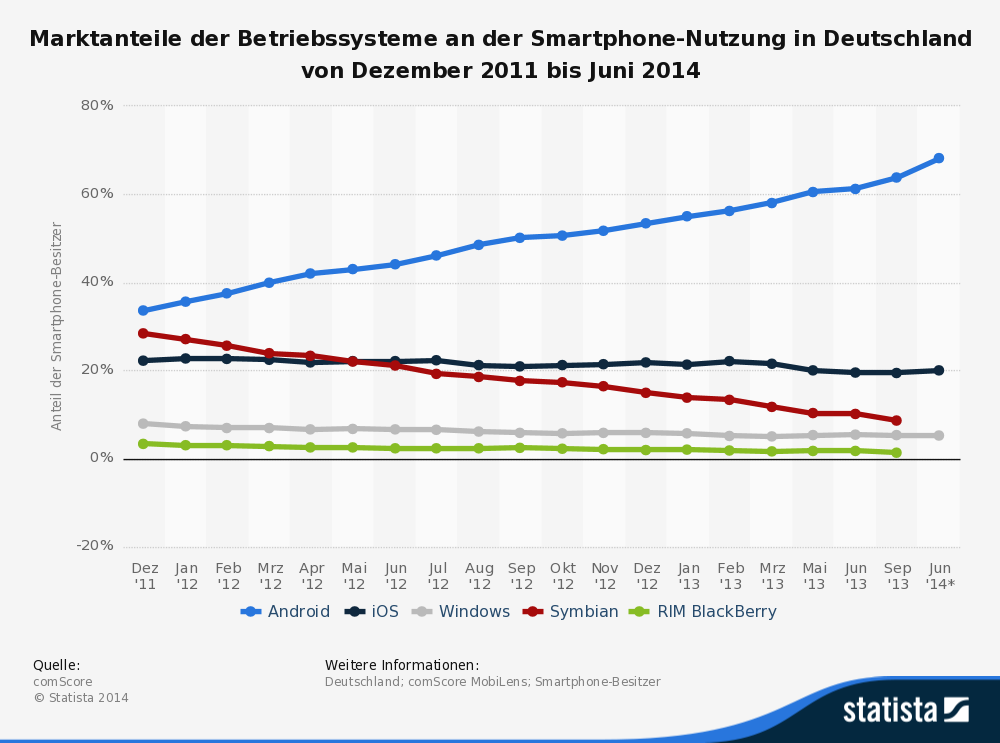
\includegraphics[width=\linewidth]{images/statistic_id170408_marktanteile-der-betriebssysteme-an-der-smartphone-nutzung-in-deutschland-bis-2014}
\caption{Marktanteile der Betriebssysteme an der Smartphone-Nutzung in Deutschland von Dezember 2011 bis Juni 2014}
\label{fig:AndroidMarktanteil}
\end{figure}
\section{Zielsetzung}\index{Zielsetzung}
Einer der WG-Mitbewohner erkl�rt sich bereit die Aufgaben des WG-Adminstrators zu �bernehmen. Dieser WG-Administrator registriert sich und legt dabei eine neue WG an. Zu seinen Aufgaben geh�rt unter anderem die Verwaltung der Mitbewohner sowie das Pflegen des Putzplans. Neue Mitbewohner m�ssen vom WG-Administrator per E-Mail in die WG eingeladen werden. F�r den Putzplan definiert er Aufgaben die in einem einstellbaren Rhythmus wiederholt werden und w�hlt zu jeder Aufgabe einen Mitbewohner aus. Nun beginnt der Rhythmus zu laufen und die Aufgaben wechseln nach Erledigung automatisch zu der n�chsten Person aus der WG. Auf dem Schwarzen Brett k�nnen Eintr�ge angezeigt, erstellt und gel�scht werden. In der Einkaufsliste k�nnen Artikel hinzugef�gt und entfernt werden. Wurde ein Artikel gekauft, kann derjenige den Artikel als gekauft markieren.
Alle �nderungen eines Mitbewohners ist f�r alle anderen Mitglieder der WG nach einer kurzen Synchronisation sichtbar.
Alle Informationen einer WG werden serverseitig in einer Datenbank und clientseitig auf dem Smartphone des Benutzers gespeichert. Bei jedem Start der App wird ein Datenabgleich der auf Client- und Serverseite gespeicherten Informationen durchgef�hrt und alle voneinander abweichenden Daten auf einer �bersichtsseite dem Benutzer als ,,Neu`` aufgelistet.
\section{�hnliche Apps}\index{�hnlicheApps}
Es gibt bereits eine Auswahl an Apps, die sich jeweils an einem kleinen Teilbereich unseres Funktionsumfanges
orientieren und dies gut umsetzen. Hierbei sind einzelne Apps f�r Einkaufslisten wie 
,,\/Shopping List``\footnote{\label{foot:shoppingList}\href{https://play.google.com/store/apps/details?id=com.fivefly.android.shoppinglist&hl=en}
{,,Shopping List`` in Google Play Store}} oder Putzpl�ne wie ,,Roomboard - Cleaning
Roster``\footnote{\label{foot:roomboard}\href{https://play.google.com/store/apps/details?id=com.roomboardapp.android&hl=en}{,,Roomboard-
Cleaning Roster`` in Google Play Store}}. Jedoch gibt es eine weitere App die sich stark an unserer Idee mit dem
Funktionumfang orientiert. Die App ,,Flatastic: Die
WG-App``\footnote{\label{foot:flatastic}\href{https://play.google.com/store/apps/details?id=com.flatastic.app}{,,Flatastic:
Die WG-App`` in Google Play Store}} bietet neben einer Einkaufsliste, einem Putzplan und einer Pinnwand zus�tzlich einen Ausgabenrechner, womit alle f�r die WG get�tigten Eink�ufe zusammengerechnet werden k�nnen.
Wir beschr�nken uns in dieser Ausarbeitung dennoch weiter auf unseren festgelegten Funktionsumfang und k�nnen uns nach der Fertigstellung nach wie vor dazu entscheiden weitere Zusatzfunktionen zu implementieren.
\inputencoding{latin1}
\chapter{Vorgehensweise}
Um m�gliche Probleme bei der Implementierung der App bereits fr�h zu identifizieren und den Arbeitsumfang der einzelnen Funktionen besser ermitteln zu k�nnen, haben wir vor Beginn der Implementierung die Risiken analysiert und uns f�r ein geeignetes Vorgehensmodell im Projektmanagement entschieden.
\section{Projektmanagement}\index{Projektmanagement}\label{sec:Projektmanagement}
Vor der eigentlichen Implementierung eines Softwareprojekts liegt oftmals mehr schriftliche Arbeit als einem lieb ist. Um in einem Team m�glichst effektiv zu arbeiten, ist es nicht nur wichtig auf das gleiche Ziel hinzuarbeiten, sondern ebenso wichtig ist es, gemeinsam den gleichen Weg zu gehen. Daf�r werden wir uns intern, sowie mit Absprache des Kunden, verschiedene Meilensteine setzen. Zu jedem abgeschlossenen Meilenstein, ob nach einem gro�en oder kleinen Fortschritt, treffen wir uns im Team gemeinsam an einem Tisch und besprechen die Ergebnisse jeder Person, um sie am Ende zusammenzutragen. Des Weiteren wird es in Absprache mit dem Kunden nach jedem abgeschlossenen gro�en Meilenstein ein Treffen mit Ihm geben. So k�nnen wir uns zu jedem Zeitpunkt des Projektes sicher sein, auf die W�nsche und Vorgaben des Kunden richtig einzugehen. Ausserdem ist er so unmittelbar mit in die Entwicklung integriert.\\
Zu Beginn m�ssen wir f�r unser Projektmanagement das passende Modell finden. Nach reichlicher �berlegung haben wir uns daf�r entschieden mit Use Cases, Mockups und Prototypen das Projekt zu beginnen. Dadurch war schnell mit dem \textit{Prototyping} das passende Modell f�r unser Vorhaben gefunden. Es gibt verschiedene Arten von \textit{Prototyping}, die alle eine andere Herangehensweise bieten. Bei n�herem Betrachten stellt sich heraus, dass das \textit{horizontale Prototyping} genau die richtige Art von \textit{Prototyping} f�r uns bietet. Dabei wird eine Ebene des Gesamtsystems m�glichst genau entworfen oder implementiert. Dies trifft perfekt auf unsere Mockups, Use-Cases und den Prototypen, den wir bereits planen, zu.\\
Da wir am Ende ein Lastenheft erstellen m�chten und wir w�hrend der Projektzeit Meilensteine definieren und zu Meilensteinsitzungen einladen werden, wird unser Management nicht nur alleine auf dem \textit{horizontalen Prototyping} basieren, sondern zus�tzlich Einfl�sse aus dem \textit{Wasserfallmodell} beinhalten. Dieses Modell zeichnet sich durch die Organisation in sogenannte Phasen aus. Dabei werden kleine Meilensteine w�hrend einer Phase und gro�e Meilensteine am Ende einer Phase definiert und in Meileinsteinsitzungen die Ergebnisse besprochen. Die wichtigsten Dokumente aus dem \textit{Wasserfallmodell} ist unter anderem das Lastenheft.\\
Damit haben wir nun als Vorgehensmodell f�r unser Projektmanagement das \textit{Horizontale Prototyping mit Einfl�ssen aus dem Wasserfallmodell}.\\

\subsection{Use-Cases}\index{Use-Cases}\label{ssec:UseCases}
Ein Use-Case (dt. Anwendungsfall) schildert auf einfache Art und Weise alle m�glichen Szenarien, die zu einem bestimmten Ziel f�hren k�nnen. Am Anfang steht ein Akteur (z.B. der Benutzer der App) der ein bestimmtes Ziel im System erreichen m�chte (z.B. das Erstellen einer Notiz). Der Use-Case beschreibt nun grob das System, die Umwelt in welchem das System arbeitet, die Anforderungen (falls gegeben) und letztendlich alle n�tigen Schritte, welche vom Benutzer get�tigt werden m�ssen, um das Ziel zu erreichen. Dazu k�nnen auch automatisierte Ereignisse vom System geh�ren.\\
Inwieweit der Use-Case ins Detail geht ist nicht definiert. Der Ersteller kann hier selbst entscheiden wie sehr eine Aktion abstrahiert werden kann und muss. Die Entscheidung kann von Use-Case zu Use-Case variieren. Es empfiehlt sich eine Vorlage mit relevanten Punkten zu erstellen, die dann bei jedem Use-Case m�glichst einheitlich ausgef�llt werden kann. Dies erleichtert im Arbeitsalltag den Gebrauch der Use-Cases.
Um eine �bersicht �ber das gesamte System aller Use-Cases zu erhalten, wird eine grafische Modellierung empfohlen. Dabei k�nnen die textbasierten Use-Cases in ein Use-Case-Diagramm vereint werden. Hierf�r ist in der Softwarentwicklung die Modellierungssprache \textit{Unified Modelling Language} (dt. vereinheitlichte Modellierungssprache, kurz: \textit{UML}) zu empfehlen. Sie wird f�r Version 2.4.1 unter anderem von der \textit{International Organization for Standardization} (dt. Internationale Organisation f�r Normung, kurz: \textit{ISO}, ISO/IEC 19505) standardisiert.\\
Ein beispielhafter Auszug aus unseren Use-Case-Diagrammen und den dazugeh�rigen Use-Cases finden Sie unter \textit{Abb.\ref{fig:UseCaseDiagrammBlackBoard} }und \textit{Abb. \ref{fig:UseCaseNotizBearbeiten}}. \\
\textit{Abb. \ref{fig:UseCaseDiagrammBlackBoard}} zeigt das Use-Case-Diagramm f�r die Funktion des Blackboards. Jedes ellipsenf�rmig eingekreiste Schlagwort steht f�r ein Use-Case. Oft ist die Wahl der Use-Cases identisch zu den der Funktionen, d.h. jede Funktion wird als Use-Case abgebildet. \\
Am Anfang steht der Benutzer der App, hier dargestellt als ein Strichm�nnchen am linken Rand des Diagramms. Der Benutzer hat die Wahl zwischen der Funktion \textit{Notiz erstellen} und \textit{Notiz bearbeiten}. Hierbei teilt sich das Diagramm in zwei Str�nge auf.\\
M�chte der Benutzer eine Notiz erstellen, wird diese am Ende des Vorgangs in der Datenbank (kurz: \textit{DB}) gespeichert. Um eine Notiz zu speichern, muss der Benutzer vorher seine Eingaben get�tigt haben. Wir haben uns daf�r entschieden die Aktionen so zu minimalisieren, dass solche Aktionen wie \textit{Text eingeben} und �hnliches als nicht relevant und gegeben anzusehen sind. Diese Aktionen fallen somit in den Use-Case \textit{Notiz erstellen} und werden nicht extra aufgef�hrt.\\
M�chte der Benutzer eine bestehende Notiz bearbeiten, so hat er dabei die M�glichkeit, die Notiz zu l�schen oder mit seinen �nderungen zu speichern.\\
Die an jeden Use-Case mit \textit{extends} angef�gte Fehlerbehandlung wird vom System automatisch ausgef�hrt, sobald ein Fehler in einem der Use-Cases auftritt. Der Fehler kann dabei durch den Benutzer, z.B. durch falsche Eingaben, sowie vom System, z.B. durch eine fehlgeschlagene Datenbankverbindung, ausgel�st werden.
\begin{figure}[H]
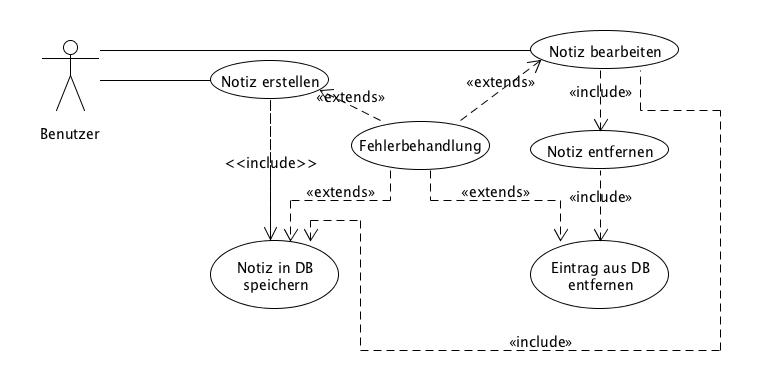
\includegraphics[width=\linewidth]{images/vorgehensweise/teamprojekt14_uc_Blackboard.jpg}
\caption{Use-Case-Diagramm f�r das Blackboard}
\label{fig:UseCaseDiagrammBlackBoard}
\end{figure}

Betrachtet man das oben eingef�gte Use-Case-Diagramm\textit{ Abb. \ref{fig:UseCaseDiagrammBlackBoard} }wird einem vermutlich auffallen, dass das Use-Case \textit{Notiz bearbeiten} komplexer erscheint als andere, jedoch genauso abstrakt dargestellt wird wie diese. Bei solchen Use-Cases, bei denen vermutlich nicht sofort jedem klar ist was im Hintergrund passiert, empfiehlt es sich eine Use-Case Beschreibung in Textform anzulegen. F�r den Fall \textit{Notiz bearbeiten} sieht unsere Beschreibung wie folgt aus.\\

\begin{figure}[H]
\centering
\begin{lstlisting}
Use-Case: Notiz bearbeiten
Ziel: Unsortierte Liste von Notizen angezeigt
Kategorie: optional (n�tzlich, nicht unbedingt notwendig)
Vorbedingung: Benutzer ist eingeloggt (in App)
Nachbedingung Erfolg: Mitteilung an Benutzer, dass Eintrag erfolgreich
Nachbedingung Fehlschlag: Mitteilung an Benutzer, dass Eintrag fehlgeschlagen
Akteure: Benutzer der App (nur registrierte WG Mitglieder)
Ausl�sendes Ereignis: Erstellung eines Eintrags von Benutzer
Beschreibung:
Notiz erstellen
1. Benutzer nimmt �nderungen an Notiz vor.
2. Benutzer m�chte Notiz speichern.
3. Notiz in Datenbank speichern.
Alternativen:
2a Benutzer entschlie�t sich die �nderungen zu verwerfen. Benutzer gelangt auf vorherigen Bildschirm
2b Benutzer entschlie�t sich die Notiz zu l�schen. Der Datenbankeintrag wird gel�scht.
\end{lstlisting}
\caption{Beschreibung des Use-Cases \textit{Notiz bearbeiten}}
\label{fig:UseCaseNotizBearbeiten}
\end{figure}

Es wird klar definiert, dass das Ziel des Use-Cases eine unsortierte Liste von Notizen sein soll. Ein Ziel muss immer
klar definiert werden. Ebenso werden \textit{Vor-} und \textit{Nachbedingungen} aufgef�hrt (falls diese vorhanden sind).
Unter \textit{Akteure} wird aufgez�hlt, wer in den Use-Case gelangen kann. In unserem Fall sind es alle Benutzer der App.
Da man die App nur als registriertes Mitglied einer WG benutzen kann, wird in den Klammern nochmals explizit darauf
hingewiesen. Die \textit{Beschreibung} schildert in Stichworten den Ablauf des Use-Cases, das hei�t man beschreibt Punkt f�r Punkt die Ereignisse die vom Benutzer sowie vom System unternommen werden um zum Ziel zu gelangen. Mit \textit{Alternativen} beschreibt man Ereignisse, die durch eine Verzweigung im Ablauf vorkommen. Diese m�ssen bereits jetzt ber�cksichtigt werden.

\subsection{Mockups}\index{Mockups}\label{ssec:Mockups}
Ein Mockup ist eine nicht lauff�hige Version einer Ebene des Gesamtsystems. Sie dient haupts�chlich zur ersten
Veranschaulichung designtechnischer Visionen. Der Begriff des Mockups wird auch ausserhalb der Softwareentwicklung gerne
f�r ma�stabsgetreue, plastisch modellierte Nachbildungen verwendet. In der Softwarentwicklung versteht man meistens eine
in Bildbearbeitungsprogrammen entworfene Vorlage der grafischen Benutzeroberfl�che. Sie soll beispielhaft das finale Produkt repr�sentieren. Im sp�teren Verlauf wird oft auf Basis der Mockups ein Screendesign entwickelt, in dem weitaus mehr Details ausgearbeitet werden. Das Screendesign dient am Ende des Projekts als Vorlage f�r den Designer, der sich bei der Gestaltung der grafischen Benutzeroberfl�che an den Vorlagen des Screendesigns orientieren muss.\\
Auch hier betrachten wir ein Beispiel aus unseren angefertigten Mockups. Wir hierf�r bewusst die Mockups f�r das
Blackboard ausgew�hlt, um zusammen mit den unter dem Kapitel \textit{\ref{ssec:UseCases} \nameref{ssec:UseCases}} in\textit{ Abb. \ref{fig:UseCaseDiagrammBlackBoard}} und \textit{Abb. \ref{fig:UseCaseNotizBearbeiten}} beschriebenen Dokumenten einen m�glichst vollst�ndigen Einblick in eine Funktion der App zu erhalten.\\
F�r die Mockups wurde das kostenfreie Programm \textit{Pencil} \cite{pencil:13} von Entwickler \textit{Evolus} verwendet. Das Programm hilft speziell bei der Gestaltung von Mockups f�r die Softwareentwicklung. Es bringt bereits viele vorgefertigte Formen und Icons aus verschiedenen Systemen mit. So ist man nach der Installation bereits in der Lage Mockups basierend auf Android Icons zu erstellen. Dieser Vorteil hat uns �berzeugt.\\
Unter Ber�cksichtigung unseres Use-Case-Diagramms Blackboard aus \textit{Abb. \ref{fig:UseCaseDiagrammBlackBoard}} ben�tigen wir drei Mockups um die relevanten Screens des Blackboards darzustellen. So w�re das ein Mockup f�r die �bersicht des Systems, eins f�r \textit{Notiz erstellen} und eins f�r \textit{Notiz bearbeiten/Notiz l�schen}.\\

\begin{figure}[H]
\centering
\includegraphics[scale=0.5]{images/vorgehensweise/mockups/blackboard.png}
\caption{Mockup 01: �bersicht Black Board}
\label{fig:Mockup01BlackBoard}
\end{figure}

In Abb. \ref{fig:Mockup01BlackBoard} ist die �bersicht zu sehen. Dies ist der Startbildschirm f�r das Blackboard. Hier
werden alle Notizen in einer Liste angezeigt. Zu jeder Notiz geh�rt ein Benutzer mit dessen Profilbild, ein Datum mit
Uhrzeit und der Text des Benutzers. Die Navigation befindet sich im Kopfbereich der App und ist f�r den Benutzer immer
zu sehen. Im unteren Bereich des Bildschirms befinden sich die speziellen Optionen der Funktion. Man kann mit einem Fingertipp auf das Textfeld eine neue Notiz erstellen und mit einem Fingertipp auf \textit{L�schen} die gew�nschten Notizen aus der Datenbank entfernen.

\begin{figure}[H]
\centering
\includegraphics[scale=0.5]{images/vorgehensweise/mockups/blackboardneuenotiz.png}
\caption{Mockup 02: Neue Notiz}
\label{fig:Mockup02BlackBoard}
\end{figure}

Will der Benutzer eine neue Notiz erstellen, so muss er von der �bersicht auf das Textfeld \textit{neue Notiz} tippen. Dann gelangt er auf das Mockup Abb. \ref{fig:Mockup02BlackBoard}, auf dem sich eine Tastatur ge�ffnet und der Button \textit{L�schen} verschwunden ist. Der Button zum L�schen von Notizen w�rde hier nur verwirren, weil die Funktion nur in der �bersicht m�glich ist. Der Button \textit{Zur�cksetzen} ist hier allerdings sehr wichtig, um dem Benutzer die M�glichkeit zu geben seinen Text mit einem Tipp auf den Button zu entfernen und gleichzeitig auf die �bersicht zur�ck zu gelangen. Ohne diese Funktion w�rde der Benutzer den Text �ber die Tastatur l�schen m�ssen und k�nnte schnell genervt sein.

\begin{figure}[H]
\centering
\includegraphics[scale=0.5]{images/vorgehensweise/mockups/blackboardnotizloeschen.png}
\caption{Mockup 03: Notiz(en) l�schen}
\label{fig:Mockup03BlackBoard}
\end{figure}

M�chte der Benutzer eine Notiz l�schen, kann er aus der �bersicht mit dem Fingertipp auf den Button \textit{L�schen} diese Funktion aktivieren (Abb. \ref{fig:Mockup03BlackBoard}). Ist er in dieser Funktion, hat er die M�glichkeit mehrere Notizen auszuw�hlen und mit einem weiteren Tippen auf \textit{L�schen} seine Auswahl aus der Datenbank zu entfernen.\\
\\
Es ist zu erkennen, dass wir uns mit dem Design der grafischen Benutzeroberfl�che an gewisse Vorlagen des Betriebssystems \textit{Android} halten m�chten. Ausserdem wird mit einem schlichten und wenig verspielten Design eine gute Lesbarkeit gew�hrleistet. Auf ein sp�teres verfeinern der Mockups durch ein Screendesign wurde bewusst verzichtet. Durch die bereits in den Mockups vorkommenden Details und farblichen Designaspekte ist eine weitere Verfeinerung in unseren Augen nicht n�tig.

\subsection{Lastenheft}\index{Lastenheft}\label{ssec:Lastenheft}
Ein Lastenheft beschreibt alle Anforderungen die der Auftraggeber an ein Projekt stellt. Es wird vom Auftraggeber erstellt und an den Auftragnehmer weitergeleitet. Der Auftragnehmer erstellt auf der Grundlage des Lastenhefts ein Pflichtenheft, in dem er seine eigenen L�sungsans�tze f�r die Anforderungen aus dem Lastenheft dem Auftraggeber pr�sentiert. Ist der Auftraggeber mit dem Pflichtenheft zufrieden, entsteht auf Grundlage dieser beiden Dokumente ein Vertrag zwischen beiden Parteien. Bei der finalen Abgabe des fertigen Produktes an den Auftraggeber, wird das Endprodukt auf Grundlage der Dokumente auf Vollst�ndigkeit gepr�ft. Kommt es zu Auseinandersetzungen, k�nnen beide Parteien auf den Mitschriften der Dokumente gegeneinander argumentieren.\\
Da wir als Team Auftraggeber und Auftragnehmer gleichzeitig sind, schreiben wir uns selbst ein Lastenheft. Dies ist uns wichtig, um w�hrend der Implementierung der App den Umfang und den Aufwand im Auge zu behalten. Wir k�nnen uns mit einem Lastenheft von Punkt zu Punkt arbeiten und bei der finalen Abgabe das Produkt gut mit den Anforderungen vergleichen. Auf ein Pflichtenheft haben wir verzichtet.\\

\begin{figure}[H]
\centering
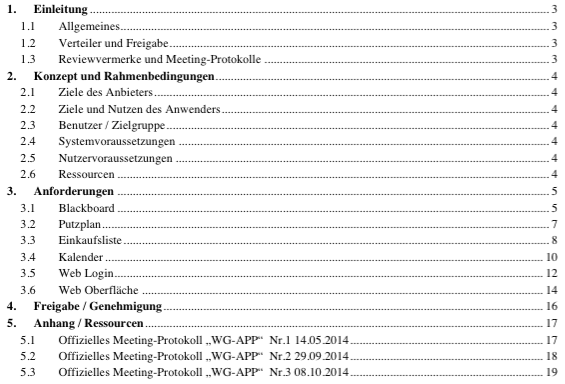
\includegraphics[width=\linewidth]{images/vorgehensweise/lastenheft/LastenheftIVZ.png}
\caption{Inhaltsverzeichnis unseres Lastenhefts}
\label{fig:LastenheftInhaltsverzeichnis}
\end{figure}

In Abb. \ref{fig:LastenheftInhaltsverzeichnis} ist das Inhaltsverzeichnis unseres Lastenhefts zu sehen und zeigt die
Struktur unseres Dokuments. Wir konzentrierten uns dabei auf das gr��te Kapitel, die \textit{Anforderungen}.  Dieses
Kapitel beschreibt alle prim�ren Funktionen der App. Dabei haben wir uns f�r \textit{Blackboard}, \textit{Putzplan},
\textit{Einkaufsliste}, \textit{Kalender}, \textit{Web Login} und \textit{Web Oberfl�che} entschieden. Jede dieser
Funktionen wird zuerst mit einem kurzen Text beschrieben. Danach kommen die Anforderungen und am Ende werden die Risiken beschreiben.\\
\\
Das gesamte Lastenheft, sowie alle Mockups, Use-Case-Diagramme und Use-Case Beschreibungen k�nnen im Anhang dieser Dokumentation nachgelesen werden.

\chapter{Anforderungen}\index{Anforderungen}\label{chp:Anforderungen}
In der Softwareentwicklung erl�utern Anforderungen alle Funktionen eines Softwareprojekts, die ein Auftraggeber vom
fertigen Produkt erwartet. Spezifiziert werden die Anforderungen im Lastenheft, welches direkt vom Auftraggeber an den
Auftragnehmer �bergeben wird.\\
Die Anforderungen werden f�r gew�hnlich in die zwei Kategorien funktional und nichtfunktional unterteilt. 
\begin{quote}
\textbf{Funktionale Anforderungen} \textit{beschreiben die Merkmale einer Funktion, also was das Produkt tun soll.}\\
\textbf{Nichtfunktionale Anforderungen} \textit{beschreiben die Eigenschaften des Produktes, also wie das Produkt etwas tun soll.}
\end{quote}
Als Beispiel nehmen wir wieder unser bekanntes Blackboard, welches wir bereits detailiert in den Kapiteln \ref{ssec:UseCases} \nameref{ssec:UseCases} sowie \ref{ssec:Mockups} \nameref{ssec:Mockups} besprochen haben. Bei unserem Blackboard haben wir die drei funktionalen Anforderungen \textit{Notiz hinzuf�gen}, \textit{Notiz bearbeiten}, \textit{Notiz l�schen} und eine nichtfunktionale Anforderung \textit{Desgin}. Betrachten wir uns die funktionale Anforderung \textit{Notiz hinzuf�gen} in Abb. \ref{fig:LastenheftAnforderungF1}.

\begin{figure}[H]
\centering
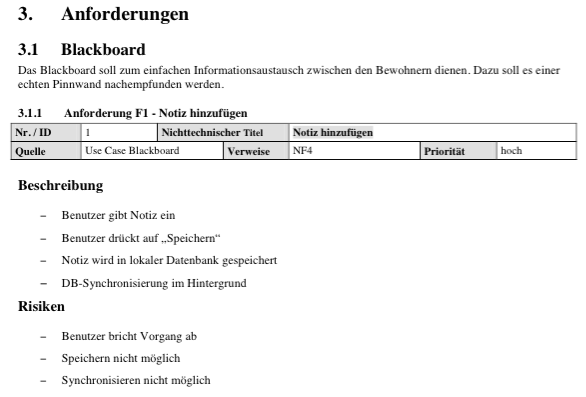
\includegraphics[width=\linewidth]{images/vorgehensweise/lastenheft/LastenheftAnforderungenBlackBoard.png}
\caption{Anforderung F1 - Notiz hinzuf�gen (Blackboard)}
\label{fig:LastenheftAnforderungF1}
\end{figure}

Zu Beginn wird die Eigenschaft jeder Anforderung in ein bis zwei kurzen S�tzen erl�utert. Daraufhin folgt eine Tabelle mit charakteristischen Merkmalen der Anforderung. Jeder Anforderung wird eine eindeutige, fortlaufende  ID zugeteilt. Au�erdem wird ein nichttechnischer Titel vergeben. Als Quelle der Anforderung dient ein anderes Dokument der Projektarbeit, im besten Fall bereits verf�gbar und f�r alle abrufbar. Meistens wird ein Dokument aus den Mockups oder Use-Cases als Quelle herangezogen. Die Verweise geben alle weiterf�hrenden Dokumente an, in denen die Anforderung weiter ausgef�hrt wird oder welche, die auf die Zusammenarbeit mit dieser Anforderung unverzichtbar sind. Letztendliche kann noch eine Priorit�t vergeben werden. Wir haben uns, mit Ausnahmen, bei vielen unserer funktionalen Anforderungen f�r eine hohe Priorit�t und bei vielen nichtfunktionalen Anforderungen f�r eine normale Priorit�t entschieden.\\
Nach der Tabelle folgt eine stichwortartige Beschreibung des grunds�tzlich vorgesehenen Ablaufes. Hierbei wird dargestellt, wie das System sowie der Benutzer agieren muss und welche Konsequenz zu erwarten sind.
Zuletzt werden alle bekannten Risiken aufgez�hlt und stichwortartig beschrieben.\\
\\

\section{Anforderungen f�r DorMApp}\label{AnforderungenDorMApp}
Alle funktionalen Anforderungen werden als \textit{Anforderung F\#} und alle nichtfunktionalen Anforderungen werden als \textit{Anforderung NF\#} gekennzeichnet.\\
Es folgen nun alle Anforderung f�r unsere App, sortiert nach den Hauptfunktionen.\\
\begin{itemize}
	\item \textbf{Blackboard}
		\begin{itemize}
			\item \textit{Anforderung F1 - Notiz hinzuf�gen}
			\item \textit{Anforderung F2 - Notiz bearbeiten}
			\item \textit{Anforderung F3 - Notiz l�schen}
			\item \textit{Anforderung NF4 - Design}			
		\end{itemize}
\end{itemize}

\begin{itemize}
	\item \textbf{Putzplan}
		\begin{itemize}
			\item \textit{Anforderung F5 - Aufgabe erledigen}
			\item \textit{Anforderung NF6 - Design}
		\end{itemize}
\end{itemize}

\begin{itemize}
	\item \textbf{Einkaufsliste}
		\begin{itemize}
			\item \textit{Anforderung F7 - Artikel hinzuf�gen}
			\item \textit{Anforderung F8 - Artikel l�schen}
			\item \textit{Anforderung F9 - Artikel gekauft}
			\item \textit{Anforderung NF10 - Design}
		\end{itemize}
\end{itemize}

\begin{itemize}
	\item \textbf{Kalender}
		\begin{itemize}
			\item \textit{Anforderung F11 - Kalendereintrag eintragen}
			\item \textit{Anforderung F12 - Kalendereintrag bearbeiten}
			\item \textit{Anforderung F13 - Kalendereintrag l�schen}
			\item \textit{Anforderung NF14 - Design}
		\end{itemize}
\end{itemize}

\begin{itemize}
	\item \textbf{Web Login}
		\begin{itemize}
			\item \textit{Anforderung F15 - Web Login}
			\item \textit{Anforderung F16 - Eingabekontrolle}
			\item \textit{Anforderung F17 - Passwort vergessen}
			\item \textit{Anforderung NF18 - Design}
		\end{itemize}
\end{itemize}

\begin{itemize}
	\item \textbf{Web Oberfl�che}
		\begin{itemize}
			\item \textit{Anforderung F19 - Benutzerverwaltung}
			\item \textit{Anforderung F20 - Terminkalenderverwaltung}
			\item \textit{Anforderung F21 - Putzplanverwaltung}
			\item \textit{Anforderung F22 - Systemeinstellungen}
			\item \textit{Anforderung NF23 - Design}
		\end{itemize}
\end{itemize}

\section{Risiken}\index{Risiken}
Risiken k�nnen den Ablauf in einer Softwarearchitektur erheblich beeinflussen. Jedes Risiko, welche vor der Implementierung nicht ber�cksichtigt wurde, kann beim Benutzer ein unkontrollierbares Verhalten verursachen. Um dies m�glichst zu vermeiden, haben wir uns bereits fr�hzeitig Gedanken um M�gliche Risiken gemacht. In einem Brainstorming kamen eine Menge Risikofaktoren zusammen, die zu einem sp�teren Zeitpunkt Probleme machen k�nnten. In unserem Lastenheft sind alle Risiken ausf�hrlich aufgelistet.
\\
\begin{itemize}
	\item \textbf{Blackboard}
		\begin{itemize}
			\item \textit{Anforderung F1 - Notiz hinzuf�gen}
				\begin{itemize}
					\item Benutzer bricht Vorgang ab
					\item Speichern nicht m�glich
					\item Synchronisieren nicht m�glich
					\\
				\end{itemize}
			\item \textit{Anforderung F2 - Notiz bearbeiten}
				\begin{itemize}
					\item Benutzer bricht Vorgang ab
					\item Speichern nicht m�glich
					\item Synchronisieren nicht m�glich
					\\
				\end{itemize}
			\item \textit{Anforderung F3 - Notiz l�schen}
				\begin{itemize}
					\item Ungewolltes L�schen
					\\
				\end{itemize}
			\item \textit{Anforderung NF4 - Design}			
				\begin{itemize}
					\item Un�bersichtliches Layout
					\item Missverst�ndliche Abl�ufe
					\\
				\end{itemize}
		\end{itemize}
\end{itemize}

\begin{itemize}
	\item \textbf{Putzplan}
		\begin{itemize}
			\item \textit{Anforderung F5 - Aufgabe erledigen}
				\begin{itemize}
					\item Fehlerhafte Synchronisierung
					\item Falsche Aufgabe ausgew�hlt
					\\
				\end{itemize}
			\item \textit{Anforderung NF6 - Design}
				\begin{itemize}
					\item Namen des Verantwortlichen zu lang und/oder in nicht darstellbarem Zeichensatz
					\item Rhythmus funktioniert nicht wie Benutzer es erwartet
					\\
				\end{itemize}
		\end{itemize}
\end{itemize}

\begin{itemize}
	\item \textbf{Einkaufsliste}
		\begin{itemize}
			\item \textit{Anforderung F7 - Artikel hinzuf�gen}
				\begin{itemize}
					\item Fehler beim Speichern in die Datenbank
					\item Der Artikel steht bereits in der Einkaufsliste, allerdings mit anderer Buchstabenformatierung (Gro�- und Kleinschreibung, Bindestrich, etc.)
					\\
				\end{itemize}
			\item \textit{Anforderung F8 - Artikel l�schen}
				\begin{itemize}
					\item Fehler beim Speichern in die Datenbank
					\item Der Artikel existiert bereits nicht mehr in der Datenbank, wird aber in der Applikation auf dem Endger�t noch angezeigt.
					\\
				\end{itemize}
			\item \textit{Anforderung F9 - Artikel gekauft}
				\begin{itemize}
					\item Fehler beim speichern in die Datenbank
					\item Der Artikel existiert bereits nicht mehr in der Datenbank, wird aber in der Applikation auf dem Endger�t noch angezeigt.
					\\
				\end{itemize}
			\item \textit{Anforderung NF10 - Design}
				\begin{itemize}
					\item Sortierung der Artikel
					\item Un�bersichtliche Aufz�hlung
					\item Schlecht leserliche Schlichtart und Schriftgr��e
					\\
				\end{itemize}
		\end{itemize}
\end{itemize}

\begin{itemize}
	\item \textbf{Kalender}
		\begin{itemize}
			\item \textit{Anforderung F11 - Kalendereintrag eintragen}
				\begin{itemize}
					\item Fehler beim Speichern in die Datenbank
					\item Titel ist zu lang
					\item Datum liegt in der Vergangenheit
					\item Datum liegt weit in der Zukunft (>50 Jahre)
					\\
				\end{itemize}
			\item \textit{Anforderung F12 - Kalendereintrag bearbeiten}
				\begin{itemize}
					\item Fehler beim Speichern in die Datenbank
					\item Titel ist zu lang
					\item Datum liegt in der Vergangenheit
					\item Datum liegt weit in der Zukunft (>50 Jahre)
					\\
				\end{itemize}
			\item \textit{Anforderung F13 - Kalendereintrag l�schen}
				\begin{itemize}
					\item Fehler beim speichern in die Datenbank
					\item Kalendereintrag existiert nicht mehr in Datenbank, wird aber noch auf dem Endger�t angezeigt
					\\
				\end{itemize}
			\item \textit{Anforderung NF14 - Design}
				\begin{itemize}
					\item Benutzer ben�tigt zu lange um sich mit dem Design zurecht zu finden
					\item Zu wenig Platz um alle Kalendereintragungen anzuzeigen
					\item Titel zu lang f�r Gesamtansicht
					\\
				\end{itemize}
		\end{itemize}
\end{itemize}

\begin{itemize}
	\item \textbf{Web Login}
		\begin{itemize}
			\item \textit{Anforderung F15 - Web Login}
				\begin{itemize}
					\item E-Mailadresse existiert nicht
					\item E-Mailadresse und/oder Passwort falsch
					\item Passwort vergessen
					\item Verbindung zum Server kann nicht hergestellt werden
					\\
				\end{itemize}
			\item \textit{Anforderung F16 - Eingabekontrolle}
				\begin{itemize}
					\item\textit{ Eingabe falscher Daten}
					\\
				\end{itemize}
			\item \textit{Anforderung F17 - Passwort vergessen}
				\begin{itemize}
					\item Missbrauch von Daten
					\\
				\end{itemize}
			\item \textit{Anforderung NF18 - Design}
				\begin{itemize}
					\item Design Gesetze nicht eingehalten (Gesetz der N�he, Gleichheit, Geschlossenheit, etc.)
					\item Gr��e der Textfelder nicht optimal
					\\
				\end{itemize}
		\end{itemize}
\end{itemize}


\begin{itemize}
	\item \textbf{Web Oberfl�che}
		\begin{itemize}
			\item \textit{Anforderung F19 - Benutzerverwaltung}
				\begin{itemize}
					\item Datenbankverbindung schl�gt fehl
					\\
				\end{itemize}
			\item \textit{Anforderung F20 - Terminkalenderverwaltung}
				\begin{itemize}
					\item Datenbankverbindung
					\\
				\end{itemize}
			\item \textit{Anforderung F21 - Putzplanverwaltung}
				\begin{itemize}
					\item Datenbankverbindung
					\\
				\end{itemize}
			\item \textit{Anforderung F22 - Systemeinstellungen}
				\begin{itemize}
					\item Datenbankverbindung
					\\
				\end{itemize}
			\item \textit{Anforderung NF23 - Design}
				\begin{itemize}
					\item Un�bersichtlich
					\\
				\end{itemize}
		\end{itemize}
\end{itemize}
Die mit Abstand anf�lligste Funktion unserer App wird die Verbindung zur Datenbank auf einen externen Server sein. Dabei kann zu jedem Zeitpunkt ein Fehler auftreten, der vom System m�glichst gut behandelt werden muss. Darum hat die Verbindung zur Datenbank mehr Aufmerksamkeit bekommen und wir haben uns daf�r entschieden einen lauff�higen Prototypen zu entwickeln. Wir haben uns bereits jetzt so stark mit der Mechanik besch�ftigt, um anstelle eines einfachen Wegwerf-Prototypen, einen im sp�teren Verlauf der Implementierung weiter zu verwendenden Prototypen entwerfen zu k�nnen.
Folgende Risiken k�nnen bei unserer Arbeit mit einer extern erreichbaren Datenbank auftreten:
\begin{itemize}
	\item Server nicht erreichbar
	\item Verbindungsabbruch durch Zusammenbruch der Internetverbindung
	\item Benutzer \textit{killt} die App w�hrend der aktiven Nutzung der Verbindung
\end{itemize}
Eine genaue Erl�uterung der Implementierung des gesamten Prototypen finden Sie im folgenden Kapitel \ref{chp:Prototyp} \nameref{chp:Prototyp}.

\chapter{Prototyp}\label{chp:Prototyp}
Um vermeidbare Verz�gerungen in der sp�teren Entwicklung m�glichst auszuschlie�en, wurde der Einsatz von Prototypen entschieden. 
Dazu werden die ben�tigten Komponenten genauer betrachtet und auf ihre Umsetzbarkeit hin untersucht. 
Bei einer Android-App, die auf Inhalte aus einer Datenbank zugreift, 
ist das die Schnittstelle zur Datenbank, beziehungsweise die Netzwerkverbindung.\\
Da eine direkte Verbindung zum Datenbankserver aus dem Android Betriebssystem nicht m�glich ist,
wurde die Authentifizierung des Benutzers als weitere Problemstelle markiert.
Den die Verwendung von Datenbankbenutzern f�llt dadurch weg und muss andersweitig gel�st werden.
Um bei diesen kritischen Stellen nicht in bredouille zu geraten, wurde daf�r ein Prototyp entwicklt.

\section{Prototyp Implementierung}\label{sect:ImplPrototyp}
Als eine einfache und schnelle Art der Umsetzung haben wir uns f�r die PHP-Variante entschieden.
Dabei werden die Daten von einem PHP-Skript aus der Datenbank gelesen und in ein JSON-Datenformat gebracht.
Dieses Objekt wird in einem HTTP-Paket an die App �bertragen.
In der App sorgt dann ein JSON-Parser f�r das Auslesen der Daten, welche anschlie�end direkt verwertet werden oder
zun�chst in der lokalen SQLite-Datenbank vorgehalten werden. \\
Alternativ zu dieser L�sung w�re ein RESTful Web Service gewesen. 
Dieser L�sungsansatz w�re jedoch mit einem gr��eren programmiertechnischen Aufwand, sowie einer umfangreicheren
Serverkonfiguration verbunden gewesen. \\
Da beide Schwerpunkte in einem Prototyp getestet wurden, wird auf eine weitere Trennung verzichtet.
\pagebreak

\subsection{Datenbankstruktur}\label{subsect:DBStruktPrototyp} 
Begonnen wurde die Umsetzung mit der Definition der Datenbankstruktur sowie deren Umsetzung.
Dazu wurden zwei einfache Tabellen angelegt. Die Tabelle \verb!tp_test! in Abb. \ref{sql:tptest} wird f�r die Schreib- und Lesevorg�nge
verwendet. Um alle n�tigen Datentypen testen zu k�nnen, wurden verschiedene Spalten verwendet. 
Dadurch konnte der sp�tere Einsatz besser simuliert werden.

\noindent
\begin{minipage}{\linewidth}
\begin{lstlisting}[caption=Aufbau der Tabelle tp\_test, captionpos=below, label=sql:tptest, language=sql, escapechar=|]
CREATE TABLE IF NOT EXISTS `test_tp` (
  `uid` VARCHAR(23) NOT NULL,
  `msg` TEXT,
  `nmbr` INT(11) DEFAULT NULL,
  `created_at` TIMESTAMP NOT NULL DEFAULT CURRENT_TIMESTAMP
) ENGINE=MyISAM DEFAULT CHARSET=utf8;
\end{lstlisting}
\end{minipage}

Um die Benutzerverwaltung f�r den Prototypen zu simulieren wurden au�erdem noch eine Tabelle \verb!users!
(siehe Abb. \ref{sql:usersTest}) angelegt.
Darin wurden Informationen zu den Benutzern hinterlegt. Zum Beispiel eine eindeutige ID, sowie Vor- und Nachname.
Zum Authentifizieren wurde die E-Mailadresse und ein beliebiges Passwort verwendet.
Um das Passwort nicht im Klartext zu speichern, wurde es zusammen mit einem Salt als Hash-Wert abgelegt.

\noindent
\begin{minipage}{\linewidth}
\begin{lstlisting}[caption=Aufbau der Tabelle users, captionpos=below, label=sql:usersTest, language=sql, escapechar=|]
CREATE TABLE IF NOT EXISTS `users` (
  `uid` int(11) NOT NULL AUTO_INCREMENT,
  `unique_id` varchar(23) NOT NULL,
  `firstname` varchar(50) NOT NULL,
  `lastname` varchar(50) NOT NULL,
  `username` varchar(20) NOT NULL,
  `wgId` int(11) NOT NULL,
  `email` varchar(100) NOT NULL,
  `encrypted_password` varchar(80) NOT NULL,
  `salt` varchar(10) NOT NULL,
  `created_at` datetime DEFAULT NULL,
  PRIMARY KEY (`uid`)
) ENGINE=MyISAM  DEFAULT CHARSET=utf8 AUTO_INCREMENT=5 ;
\end{lstlisting}
\end{minipage}

\subsection{PHP-Skripte}\label {subsect:PHPrototyp}
Der Aufbau der PHP-Schnittstelle ist simpel umgesetzt, da nicht viele Funktionen f�r den Prototyp ben�tigt werden.
Trotzdem wurde auf eine �bersichtliche Datei- und Ordnerstruktur, als auch auf einen modularen Aufbau geachtet.
Wie in Abbildung \ref{dirtree:phpPrototyp} \nameref{dirtree:phpPrototyp} zu sehen, wurde der Aufbau zun�chst in zwei Kategorien aufgeteilt.
Funktionen, die direkt auf der Datenbank ausgef�hrt werden, sowie das Verbinden und Bereitstellen des Datenbankobjekts
�bernehmen, sind im Ordner \verb!php/include! untergebracht.
Alle weiteren Funktionen die aus der App heraus erreichbar sein sollen, befinden sich im Hauptordner \verb!php!.

\begin{figure}[H]
  \centering
  \begin{minipage}{1.0\textwidth} \small
    \dirtree{%
      .1 php.
        .2 include.
          .3 config.php \ldots{} \begin{minipage}[t]{5cm}
                                Verbindungsparameter f�r die Datenbank{.}
                               \end{minipage}.
          .3 DB\_Connect.php \ldots{}
                               \begin{minipage}[t]{5cm}
                                 Funktionen zum Aufbau und dem Bereitstellen der Datenbankverbindung{.}
                               \end{minipage}.
          .3 DB\_Functions.php \ldots{} \begin{minipage}[t]{5cm}
                                  Methoden f�r Datenbankoperationen; zum Beispiel getTable{.}
                                \end{minipage}.
        .2 db.php \ldots{} \begin{minipage}[t]{5cm}
                                  Verarbeitung des HTTP-Requests, auswerten der Anfrage, sammeln der Daten und
                                  abschlie�end Daten verpacken und an Client zur�cksenden{.}
                                \end{minipage}.
        .2 login.php \ldots{} \begin{minipage}[t]{5cm}
                                  Authentifizieren des Benutzers{.}
                                \end{minipage}.
    }
  \end{minipage}
  \caption{Struktur der PHP-Skripte im Dateisystem}
  \label{dirtree:phpPrototyp}
\end{figure}

Die vollst�ndigen Skripte befinden sich im Anhang und werden hier nur in Ausz�gen dargestellt. \\
Der Ablauf zum Aufrufen der einzelnen PHP-Funktionen ist immer derselbe. 
Dazu wird ein POST-Request an den Server geschickt, der die entsprechende Ressource, in diesem Fall entweder
\verb!db.php! oder \verb!login.php!, anfordert. Als POST-Parameter werden neben den Werten f�r die Funktion, 
zum Beispiel E-Mailadresse und Passwort f�r den Login, noch ein TAG-Parameter angeh�ngt. 
Der TAG-Parameter ist f�r den Login-Prozess zum Beispiel leer, zum �ndern des Passworts kann dazu \verb!chgpass!
eingesetzt werden. Nachdem die zum TAG passende Funktion gefunden wurde, werden die �bertragenen Werte ausgelesen und
entsprechend verarbeitet. \\
Eine wichtige Funktion der PHP-Skripte ist der Login bzw. die Authentifizierung des Benutzers. \\*
Dazu wird die Adresse \verb!http://test.app1.raschel.org/php/db.php! mit den Parametern \verb!TAG=''!,
\verb!EMAIL=`ritzels@fh-trier.de'! und \verb!PASSWORD=`ritzels'! aufgerufen (vgl. Abb. \ref{php:loginProto}).
Sind alle Parameter korrekt �bertragen worden, wird die Funktion \verb!getUserByEmailAndPassword($email, $password)!, die sich im Skript \verb!DB\_Functions.php! befindet, aufgerufen. Zum Authentifizieren wird aus der Datenbank der zur
E-Mailadresse passende Datensatz geladen, siehe Auszug \ref{php:dbFuncProto}.
Das in der Datenbank gespeicherte \verb!SALT! wird mit dem �bertragenen Passwort an die Funktion
\verb!checkhashSSHA($salt, $password)! �bergeben, welche den Hash aus \verb!SALT! und Passwort bildet und zur�ckgibt.
Dieser generierte Hash wird dann mit dem in der Datenbank gespeichertem \verb!encrypted_password! verglichen. Stimmen
die beiden Hashs �berein, wird der geladene Datensatz an die Login-Funktion zur�ckgeliefert, ansonsten liefert die
Funktion \\* \verb!getUserByEmailAndPassword() -> false!.

\noindent
\begin{minipage}{\linewidth}
\begin{lstlisting}[caption=Auszug aus login.php, captionpos=below, label=php:loginProto, language=php, escapechar=|]
<?php
[|\ldots{}|]
if (isset($tag) && $tag != `') {
  require_once 'include/DB_Functions.php';
  $db = new DB_Functions();
  $response = array("tag" => $tag, "success" => 0, "error" => 0);
  if ($tag == 'login') {
  $email = $_POST['email'];
  $password = $_POST['password'];
  $user = $db->getUserByEmailAndPassword($email, $password);
  if ($user) {
    $response["success"] = 1;
    $response["user"]["user_id"] = $user["user_id"];
    $response["user"]["wg_id"] = $user["wg_id"];
    $response["user"]["crea"] = $user["crea"];
    echo json_encode($response);
  } else {
    $response["error"] = 1;
    $response["error_msg"] = $IncorrectEMail;
    echo json_encode($response);
  }
}
else if ($tag == 'chgpass') {
[|\ldots{}|]
\end{lstlisting}
\end{minipage}

\noindent
\begin{minipage}{\linewidth}
\begin{lstlisting}[caption=Auszug aus DB\_Functions.php, captionpos=below, label=php:dbFuncProto, language=php, escapechar=|]
[|\ldots{}|]
private $db;
function __construct() {
  require_once 'DB_Connect.php';
  $this->db = new DB_Connect();
  $this->db->connect();
}
public function getUserByEmailAndPassword($email, $password) {
  $resultSQL = mysql_query("SELECT * FROM user WHERE email = '$email'")
      or die(mysql_error());
  $no_of_rows = mysql_num_rows($resultSQL);
  if ($no_of_rows > 0) {
    $result = mysql_fetch_array($resultSQL);
    $salt = $result['salt'];
    $encrypted_password = $result['passwort'];
    $hash = $this->checkhashSSHA($salt, $password);
    if ($encrypted_password == $hash) {
      return $result;
    }
[|\ldots{}|]
\end{lstlisting}
\end{minipage}

%Im Kapitel ref{sec:App} werden noch weitere Funktionen erl�utert, die in diesem Kapitel noch keine Rolle spielen.
Die Skripte befinden sich in vollem Umfang als Anhang an diese Dokumentation.
\pagebreak

\subsection{Prototyp-App}\label{subsect:PrototypApp}
Die Implementierung der Prototyp-App wurde in zwei Projekte aufgeteilt. In dem Projekt \verb!DatabaseConnectionLib!
wurden die Funktionen zum Schreiben und Lesen der MySQL-Datenbank ausgelagert, da diese mit Sicherheit f�r die sp�tere
Implementierung wieder Verwendung finden werden. Das Anzeigen und Manipulieren der Daten wurde im Projekt
\verb!DBPrototyp! zusammengefasst.

\subsubsection*{DBPrototyp}\label{subsub:DBPrototyp}
Das Projekt wurde noch in der Entwicklungsumgebung Eclipse erstellt und umfasst deshalb eine etwas tiefere
Ordnerhirarchie. Da nicht alle f�r diese Implementierung relevant sind, werden nur die wichtigsten Ordner und Dateien
n�her erl�utert. \\
Der Ordnerbaum in Abb. \ref{dirtree:dbProto} zeigt die wichtigen Ordner und Dateien, und erl�utert kurz deren Funktion.

\begin{figure}[H] 
  \centering
  \begin{minipage}{1.0\textwidth} \small
    \dirtree{%
      .1 DBPrototyp.
        .2 src.
          .3 de.hst.teamprojekt.dbprototype.
            .4 LoginActivity.java \ldots{} \begin{minipage}[t]{8cm}
                                 Java-Klasse mit den Funktionen zum Login{.}
                               \end{minipage}.
            .4 MainActivity.java \ldots{} \begin{minipage}[t]{8cm}
                                 Java-Klasse mit den Funktionen zum Lesen und Schreiben der Daten{.}
                                \end{minipage}.
        .2 res.
          .3 layout. 
            .4 activity\_login.xml \ldots{} \begin{minipage}[t]{8cm}
                                  Layout-Datei f�r die Login-Oberfl�che{.}
                                \end{minipage}.
            .4 activity\_main.xml \ldots{} \begin{minipage}[t]{8cm}
                                  Layout-Datei f�r die Standard-Oberfl�che{.}
                                \end{minipage}.
          .3 menu \ldots{} \begin{minipage}[t]{8cm}
                                  Beinhaltet die Men�struktur der einzelnen Oberfl�chen{.}
                                \end{minipage}.
          .3 values \ldots{} \begin{minipage}[t]{8cm}
                                 Beinhaltet XML-Dateien, in denen Werte hinterlegt werden k�nnen die nicht im Quellcode
                                 sein sollten{.}
                                \end{minipage}.
        .2 AndroidManifest.xml \ldots{} \begin{minipage}[t]{8cm}
                                  Allgmeine Parameter der App, wie unterst�tzte API-Version oder ben�tigte Ressourcen,
                                  bzw{.} Erlaubnis f�r die Ressourcen{.}
                                \end{minipage}.
    }
  \end{minipage}
  \caption{Verzeichnisstruktur des DBPrototyp-Projekts}
  \label{dirtree:dbProto}
\end{figure}


%%%%%%%%%%%%%%%%%%%%%
\begin{comment}
\paragraph{Android Manifest}\label{para:ProtoManifest}
In der \verb!AndroidManifest.xml! werden grundlegende Parameter f�r die App festgelegt.
Dabei sind f�r diesen Prototyp zun�chst nur die Elemente \verb!uses-permission!, durch das die verwendeten Ressourcen
angegeben werden k�nnen, sowie \verb!activity!, �ber das das Betriebssystem erf�hrt welche Activity als erste gestartet
wird und welche au�erdem noch verwendbar sind. \\
Die genaue Umsetzung dieser Einstellungen und welche weiteren Elemente verwendet wurden, k�nnen aus der angeh�ngten
AndroidManifest.xml entnommen werden.

\paragraph{Menu und Values}\label{para:ProtoMenuValues}
Im Ordner \verb!menu! werden die Men�punkte der einzelnen Aktivit�ten deklariert.
Die Funktion hinter den einzelnen Punkten wird dann in der jeweiligen Aktivity-Klasse implementiert.
Zum Beispiel wurde f�r den Login ein Men�punkt in der \verb!MainAcitivity! angelegt.
In der \verb!main.xml! wird daf�r ein neues Element erstellt mit Attribute f�r den Namen, die Sortierung oder welche
Kategorie dieser Men�punkt angeh�rt (vgl. \ref{xml:mainMenuProto}).

\noindent
\begin{minipage}{\linewidth}
\begin{lstlisting}[caption=Auszug aus menu/main.xml, captionpos=below, label=xml:mainMenuProto, language=xml, escapechar=|]
[|\ldots{}|] 
<item android:id="@+id/action_settings" android:orderInCategory="100"
  android:title="@string/action_settings" app:showAsAction="never" 
  android:menuCategory="system"
  android:actionLayout="@layout/activity_login" />
[|\ldots{}|]
\end{lstlisting}
\end{minipage}

Um diesen Men�punkt noch mit einer Funktion zu versehen, muss in der \verb!MainActivity.java! \ref{java:MainActivityProto} das Men� zun�chst generiert werden
(Zeile ~\ref{line:onCreateOptionsMenuProto}). Wird der Eintrag ausgew�hlt, ruft ein Listener die Methode \verb!onOptionsItemSelected!
~\ref{line:onOptionsItemSelProto} auf, in welcher dann mittels dem �bergebenen \verb!MenuItem!-Objekt die gew�nschte
Operation, in diesem Fall das Starten der \verb!LoginActivity.java!, ausgef�hrt wird.

\noindent
\begin{minipage}{\linewidth}
\begin{lstlisting}[caption=Auszug aus MainActivity.java, captionpos=below, label=java:MainActivityProto, language=java, escapechar=|]
[|\ldots{}|]
@Override
public boolean onCreateOptionsMenu(Menu menu) { |\label{line:onCreateOptionsMenuProto}|
  // Inflate the menu; this adds items to the action bar if it is present.
  getMenuInflater().inflate(R.menu.main, menu);
  return true;  }

@Override
public boolean onOptionsItemSelected(MenuItem item) { |\label{line:onOptionsItemSelProto}|
  // Handle action bar item clicks here. The action bar will
  // automatically handle clicks on the Home/Up button, so long
  // as you specify a parent activity in AndroidManifest.xml.
  int id = item.getItemId();
  if (id == R.id.action_settings) {
      Intent loginIntent = new Intent(this, LoginActivity.class);
      loginIntent.putExtra(Constants.EXTRA_EMAIL, creds.getUname());
      startActivity(loginIntent);
      return true;  }
  return super.onOptionsItemSelected(item);  }
[|\ldots{}|]
\end{lstlisting}
\end{minipage}

weiter ausf�hren?

\paragraph{Oberfl�che}\label{para:GUIProto}
Im Ordner \verb!layout! befinden sich xml-Dateien, die das Layout definieren.
Beim Start der App wird, wie in der Manifest-Datei angegeben, die MainActivity geladen, in der die Methode
\verb!onCreate()! ausgef�hrt wird. 
\end{comment}
%%%%%%%%%%%%%%%%%%%%%


F�r die Funktion des Prototypen und das Umsetzen der definierten Schwerpunkte sind in diesem Projekt die beiden Klassen
\verb!LoginActivity.java! und \verb!MainActivity.java! von Bedeutung.
Beim Start der App wird zun�chst die \verb!MainActivity.java! mit dem Layout \verb!activity_main.xml! geladen (siehe Abb. \ref{pic:MainActivityProto}).
Das geschieht in Zeile \ref{line:setContentViewProto} durch \verb!setContentView(R.layout.activity_main)! in der \verb!onCreate()! Methode.

\begin{figure}[H]
  \centering
  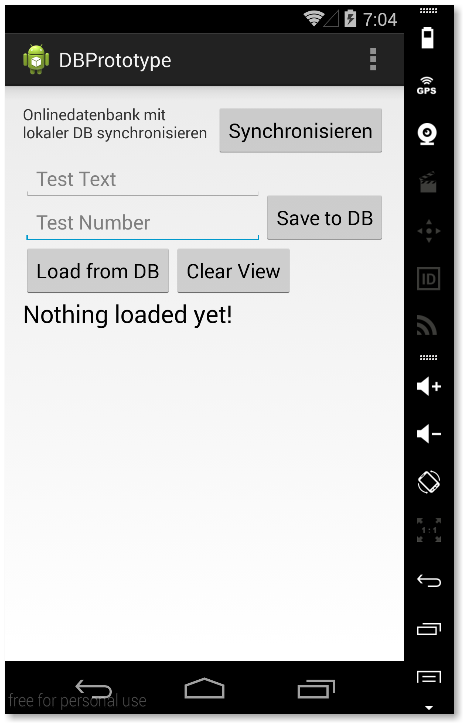
\includegraphics[width=0.4\textwidth]{images/prototyp/MainActivityEmpty.png}
  \caption{Start-Oberfl�che}
  \label{pic:MainActivityProto}
\end{figure}

Ist alles vollst�ndig geladen, kann man sich �ber das Men� anmelden. Daf�r wird in der \verb!onOptionsItemSelected(MenuItem item)! ein
\verb!startActivity()! aufgerufen, welches die \verb!LoginActivity.java! startet (siehe Abb.
\ref{pic:LoginActivityProto}).

\begin{figure}[H]
  \centering
  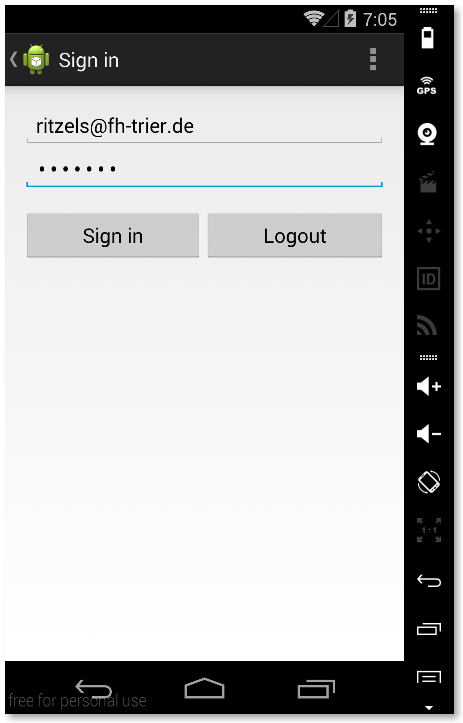
\includegraphics[width=0.4\textwidth]{images/prototyp/LoginActivity.png}
  \caption{Login-Oberfl�che}
  \label{pic:LoginActivityProto}
\end{figure}

Nach der erfolgreichen Authentifizierung wird �ber den Button \texttt{Synchronisieren} die Funktion
\verb!synchronizeDbs(View view)! in Zeile \ref{line:synchDbsProto} aufgerufen. \\
Dies generiert ein Objekt der Klasse \verb!SyncRemoteDatabase.java! (siehe Abb. \ref{java:SyncRemoteDBProto}). Dabei handelt es sich um eine von \verb!AsyncTask!
abgeleitete Klasse, welche die Testdaten �ber das PHP-Skript aus der Datenbank abruft und anschlie�end in die lokale
\verb!SQLite!-Datenbank schreibt. Diese Klasse wird in dem Kapitel \ref{subsub:DBConLibProto} \verb!DBConnectionLib! genauer erl�utert.

\noindent
\begin{minipage}{\linewidth}
\begin{lstlisting}[caption=Auszug aus der MainActivity.java, captionpos=below, label=java:MainActivityProto, language=java, escapechar=|]
[|\ldots{}|]
@Override
protected void onCreate(Bundle savedInstanceState) {
  super.onCreate(savedInstanceState);
  setContentView(R.layout.activity_main); |\label{line:setContentViewProto}|
[|\ldots{}|]
public void synchronizeDbs(View view) { |\label{line:synchDbsProto}|
  {|\ldots{}|}
  SyncRemoteDatabase queryTask = 
    new SyncRemoteDatabase(MainActivity.this, this.creds);
  queryTask.execute(Constants.TABLE_TEST);
}
[|\ldots{}|]
\end{lstlisting}
\end{minipage}

Wurden die Tabellen erfolgreich synchronisiert, k�nnen �ber die beiden Felder Testwerte eingegeben werden. Durch einen
Klick auf den Button \texttt{Save to DB} werden die Daten zun�chst in der Methode \verb!saveToDb(View view)!(Zeile ~\ref{line:saveToDbProto})
in \textsl{BasicNameValuePair}-Objekte �berf�hrt (Zeile \ref{line:tableNameProto} - \ref{line:testNumberProto}).
Zum Speichern werden diese Objekte an eine Instanz der Klasse
\verb!InsertIntoDatabase.java! �bergeben. Diese ist, wie die Klasse \verb!SyncRemoteDatabase.java!, eine Subklasse von
\verb!AsyncTask! und wird ebenfalls im Kapitel \ref{subsub:DBConLibProto} genauer erkl�rt.
Zum Anzeigen der lokalen Tabelleninhalte kann der Button \texttt{Load from DB} bet�tigt werden, wodurch die Funktion
\verb!loadFromDb(View view)! ausgef�hrt wird. Dabei werden die Daten zun�chst in einem \textsl{Cursor}-Objekt
bereitgestellt, welches vom \texttt{DatabaseHandler} (siehe Abb. \ref{java:DBHandlerProto}) bereitgestellt wird (vgl. Zeile
\ref{line:CursorProto}). Die Darstellung wird durch eine \textsl{ListView} �bernommen, die im
Layout der Aktivit�t hinterlegt und �ber den Befehl \\* \verb!findViewById(R.id.listView1)! in Zeile \ref{line:findListViewProto} 
referenziert wurde. Um den \textsl{Cursor} in der \textsl{ListView} anzeigen zu k�nnen, muss dieser in einem
\textsl{SimpleCursorAdapter} f�r die \textsl{ListView} zug�nglich gemacht werden. Dazu wird in Zeile
\ref{line:SiCuAdProto} dem Konstruktor des \textsl{SimpleCursorAdapter} zun�chst der aktuelle \textsl{Context}, das
gew�nschte Layout der einzelnen Zeilen (\verb!R.Layout.list_item!) sowie der \textsl{Cursor} \verb!result!, �bergeben.
Damit der Adapter wei�, welche Werte er in welche \textsl{TextView} packen soll, werden dem Konstruktor noch \verb!from!
und \verb!to! �bergeben. 

\noindent
\begin{minipage}{\linewidth}\begin{lstlisting}[caption=Auszug aus der MainActivity.java, captionpos=below, label=java:MainActivityProto3, language=java, escapechar=|]
[|\ldots{}|]        
public void saveToDb(View view) { |\label{line:saveToDbProto}|
  {|\ldots{}|}
  BasicNameValuePair tablename = 
    new BasicNameValuePair("table", Constants.TABLE_TEST); |\label{line:tableNameProto}|
  BasicNameValuePair testText = new BasicNameValuePair("msg", 
        ((EditText) findViewById(R.id.editTestText)).getText().toString());
  BasicNameValuePair testNumber = new BasicNameValuePair("nmbr", ((EditText)
  findViewById(R.id.editTestNmbr)).getText().toString()); |\label{line:testNumberProto}|

  InsertIntoDatabase saveTask = 
    new InsertIntoDatabase(MainActivity.this, this.creds);
  saveTask.execute(tablename, testText, testNumber);
}
public void loadFromDb(View view) {
  {|\ldots{}|}
  Cursor result = db.getTestRow(1); |\label{line:CursorProto}|

  if (result.getCount() > 0) {
      String[] from = new String[]
      { Constants.KEY_UID, Constants.KEY_TEST_STRING, 
        Constants.KEY_TEST_INT, Constants.KEY_CREATED_AT };

      int[] to = new int[]
      { R.id.uid, R.id.msg, R.id.nmbr, R.id.created_at };

      SimpleCursorAdapter sca = new SimpleCursorAdapter
        (this, R.layout.list_item, result, from, to, 0); |\label{line:SiCuAdProto}|
      ListView lv = (ListView) findViewById(R.id.listView1); |\label{line:findListViewProto}|
      lv.setAdapter(sca);
      lv.setVisibility(ListView.VISIBLE);
  {|\ldots{}|}
}
public void clearResultListVew(View view) { |\label{line:clearLVProto}|
  TextView txtView = (TextView) findViewById(R.id.textView2);
  txtView.setText(R.string.txtNothingLoaded);
  txtView.setVisibility(TextView.VISIBLE);
  ListView lv1 = (ListView) findViewById(R.id.listView1);
  lv1.setAdapter(null);
  lv1.setVisibility(ListView.INVISIBLE);
}
[|\ldots{}|]
\end{lstlisting}
\end{minipage}

Dabei handelt es sich bei dem Objekt \verb!from! um eine \textsl{String}-Liste mit den Namen der Tabellenspalten. Die
\textsl{int}-Liste \verb!to! enth�lt die IDs der \textsl{TextView}s im verwendeten Zeilenlayout. Die Reihenfolge muss
dabei beachtet werden. Abschlie�end erh�lt der Konstruktor noch eine Flag mit der das Verhalten bei �nderung der
Datengrundlage gesteuert wird. Dieser Adapter wird mittels dem Befehl \verb!.setAdapter(sca)! der \textsl{ListView}
�bergeben. Wodurch nun die Daten auf der Oberfl�che sichtbar werden. \\*

Zum Leeren der \textsl{ListView} wird der Button \texttt{Clear View} gedr�ckt, wodurch mittels der Methode
\textsl{clearResultListView(View view)} in Zeile \ref{line:clearLVProto} die \textsl{ListView} vom Adapter
getrennt und unsichtbar gemacht wird.
\pagebreak

\subsubsection*{DatabaseConnectionLib}\label{subsub:DBConLibProto}
Das Projekt \verb!DatabaseConnectionLib! wurde, wie bereits erw�hnt, zum Auslagern von wiederverwendbaren Modulen erstellt. 
Aus diesem Grund befinden sich darin keine Layout, Values oder �hnliche Ressourcen die zur Darstellung und Bedienung
n�tig sind. Da die Ordner- und Dateistruktur der Projekte nahezu identisch ist, wird von einer weiteren Auff�hrung
dieser Details abgesehen. In diesem Kapitel werden dementsprechend nur die Klassen n�her erl�utert, die im Kapitel
\nameref{subsub:DBPrototyp} \ref{subsub:DBPrototyp} schon erw�hnt wurden.

\paragraph{Klasse SyncRemoteDatabase.java}\label{para:SyncRemoteDBProto}
Instanziiert wird diese Klasse in der \verb!MainActivity.saveToDb()! Funktion. Um die Bedienbarkeit der Oberfl�che nicht
zu verhindern oder die App zum Einfrieren zu bringen, was durch eine langanhaltende Operation passieren k�nnte, wurde
diese Klasse von der \verb!AsyncTask!-Klasse abgeleitet. Diese erm�glicht eine komfortable M�glichtkeit mit Threads zu
arbeiten und somit die Operationen vom GUI-Thread auszulagern. Der Vorteil gegen�ber dem Ausf�hren eines einfachen
\texttt{Runnable}-Objekts in einem gesonderten Thread ist, dass die \verb!AsyncTask!-Klasse ableitbare Methoden besitzt
mit denen bevor und w�hrend der Thread l�uft, sowie nach dem Beenden des Threads, Operationen ausgef�hrt werden k�nnen.
Im Fall der \verb!SyncRemoteDatabase!-Klasse wird vor dem Ausf�hren des Task, mittels der Methode \textsl{onPreExecute()}, 
ein \texttt{ProgressDialog} erstellt (vgl. Zeilen \ref{line:onPreExecProto} ff.). 
Anschlie�end wird im asynchronen Teil \textsl{doInBackground(String\ldots{} params)}, die Funktion
\verb!syncRemoteTable(creds, params[0])!(Zeile \ref{line:syncRemTabProto}) aufgerufen und das damit erzeugte \texttt{JSONObject}-Objekt
an die Methode \textsl{onPostExecute(JSONObject json)}(Zeile \ref{line:postExecProto}) �bergeben.
Da diese Methode, wie die \textsl{onPreExecute}, im GUI-Thread l�uft, kann der \texttt{ProgressDialog} mit einer neuen
Nachricht versehen werden (Zeile \ref{line:pDialogPostProto}) und die erhaltenen Daten aus dem \texttt{JSONObject}-Objekt
extrahieren (Zeile ~\ref{line:parseJsonProto}). Im selben Schritt werden die Testdaten der Testtabelle als neuen
Datensatz angef�gt (siehe Zeile ~\ref{line:addTestRowProto}). \\

\noindent
\begin{minipage}{\linewidth}
\begin{lstlisting}[caption=Auszug aus SyncRemoteDatabase.java, captionpos=below, label=java:SyncRemoteDBProto, language=java, escapechar=|]
[|\ldots{}|]        
@Override
protected void onPreExecute() { |\label{line:onPreExecProto}|
  super.onPreExecute();
  pDialog = new ProgressDialog(appContext);
  pDialog.setTitle("Contacting Servers");
  pDialog.setMessage("Query database ...");
  pDialog.setIndeterminate(false);
  pDialog.setCancelable(true);
  pDialog.show();
};
@Override
protected JSONObject doInBackground(String... params) { 
/** {|\ldots{}| **/
  JSONObject json = userFunction.syncRemoteTable(creds, params[0]); |\label{line:syncRemTabProto}|
  return json;
}
@Override
protected void onPostExecute(JSONObject json) { |\label{line:postExecProto}|
/** {|\ldots{}| **/
  pDialog.setMessage("Loading Test Data"); |\label{line:pDialogPostProto}|
  pDialog.setTitle("Getting Data");
  JSONArray json_array = json.getJSONArray("result");
  /** {|\ldots{}|} **/
    db.dropSyncTable();
    for (int i = 0; i < Integer.parseInt(res); i++) { |\label{line:parseJsonProto}|
      JSONObject json_data = json_array.getJSONObject(i);
      db.addTestRow(json_data.getInt(Constants.KEY_UID), |\label{line:addTestRowProto} |
        json_data.getString(Constants.KEY_TEST_STRING),
        json_data.getInt(Constants.KEY_TEST_INT),
        json_data.getString(Constants.KEY_CREATED_AT)); 
    }
[|\ldots{}|]
\end{lstlisting}
\end{minipage}

Die angesprochene Funktion \textsl{syncRemoteTable()} befindet sich in der Klasse \verb!UserFunctions.java!
(siehe Listing \ref{java:UsrFuncsProto}). Darin wurden die Methoden zusammengefasst, die vom Benutzer oder mit dem Benutzer
zusammenh�ngen. Neben den Methoden \textsl{loginUser({\ldots})} und \textsl{loggedInUser({\ldots})}, enth�lt sie auch
die Methode \textsl{syncRemoteTable(AuthCredentials creds, String table)} (Zeile \ref{line:synRemTableProto}), die zum Abrufen
der Testdaten aus der MySQL-Datenbank verwendet wird. \\*
Dazu werden zun�chst die \emph{POST}-Parameter in eine Liste aus \texttt{BasicNameValuePair}-Objekten gepackt, wie in
den Zeilen \ref{line:POSTParaVonProto} bis \ref{line:POSTParaBisProto} zu sehen.\\

\noindent
\begin{minipage}{\linewidth}
\begin{lstlisting}[caption=Auszug aus UserFunctions.java, captionpos=below, label=java:UsrFuncsProto, language=java, escapechar=|]
[|\ldots{}|]        
public JSONObject syncRemoteTable(AuthCredentials creds, String table) { |\label{line:synRemTableProto}|
  List<BasicNameValuePair> params = new ArrayList<BasicNameValuePair>(); |\label{line:POSTParaVonProto}|
  params.add(new BasicNameValuePair("tag", syncTag));
  params.add(new BasicNameValuePair("email", creds.getEmail()));
  params.add(new BasicNameValuePair("password", creds.getPassword()));
  params.add(new BasicNameValuePair("table", table)); |\label{line:POSTParaBisProto}|
  JSONObject json = jsonParser.getJSONFromUrl(syncUrl, params);  |\label{line:getJsonFromUrlProto}|
  return json;
}
[|\ldots{}|]
\end{lstlisting}
\end{minipage}

Die so verpackten Parameter werden schlie�lich an den \verb!JSONParser! (siehe Listing \ref{java:JSONParserProto}) �bergeben.
Die darin enthaltene Funktion \\* \textsl{getJSONFromUrl(String url, List<BasicNameValuePair> params)} der
\nameref{line:getJsonFromUrlProto} schickt die erhaltenen Attribute mittels \texttt{DefaultHttpClient()}- und
\texttt{HttpPost}-Objekt zur angegebenen \emph{url} (Zeile \ref{line:httpConnection} ff).
Die Serverantwort, die vom Socket �ber den \texttt{InputStream} erreichbar wird, wird durch einen
\texttt{BufferedReader} lesbar. Der \texttt{BufferedReader} ist hier besonders geeignet, da dadurch ein zeilenweises
Lesen erm�glicht wird, was bei \emph{HTTP}-Kommunikationen das Standardverfahren ist (Zeile \ref{line:bufRdrProto} und
\ref{line:readLineProto}). Jede Zeile wird an einen \textsl{StringBuilder} geh�ngt und nach dem Lesen der
letzten Zeile von einem \verb!String! (Zeile \ref{line:sb.toString(Proto)}) in das gew�nschte \textsl{JSONObject} umgewandelt.\\

\noindent
\begin{minipage}{\linewidth}
\begin{lstlisting}[caption=Auszug aus JSONParser.java, captionpos=below, label=java:JSONParserProto, language=java, escapechar=|]
public JSONObject getJSONFromUrl(String url, 
    List<BasicNameValuePair> params) {
[|\ldots{}|]        
  DefaultHttpClient httpClient = new DefaultHttpClient(); |\label{line:httpConnection}|
  HttpPost httpPost = new HttpPost(url);
  httpPost.setEntity(new UrlEncodedFormEntity(params));
  HttpResponse httpResponse = httpClient.execute(httpPost);
  HttpEntity httpEntity = httpResponse.getEntity();
  is = httpEntity.getContent();
[|\ldots{}|]
  BufferedReader reader =
    new BufferedReader(new InputStreamReader(is, "iso-8859-1"), 8); |\label{line:bufRdrProto}|
  StringBuilder sb = new StringBuilder();
  String line = null;
  while ((line = reader.readLine()) != null) { |\label{line:readLineProto}|
    sb.append(line + "\n");
  }
  is.close();
  json = sb.toString(); |\label{line:sb.toString(Proto)}|
[|\ldots{}|]
else {
  jObj = new JSONObject(json); |\label{line:newJSONObjectProto}|
}
[|\ldots{}|] 
\end{lstlisting}
\end{minipage}

Die so verpackte Tabelle, wird dann mit einer \verb!for!-Schleife (Listing \ref{java:SyncRemoteDBProto} \# \ref{line:parseJsonProto}) in die einzelnen Zeilen zerlegt und von der Funktion
\textsl{addTestRow(\ldots{})} (Zeile \ref{line:addTstRwProto}) in die lokale \verb!SQLite!-Datenbank geschrieben
(Listing \ref{java:SyncRemoteDBProto} \# \ref{line:addTestRowProto}). Dazu werden die einzelnen Werte in zun�chst mit den zugeh�rigen Spaltennamen in ein
sogenanntes \texttt{ContentValues}-Objekt geschrieben, was im Groben einer Tabellenzeile entspricht.
Eine solche Kapselung ist theoretisch nicht n�tig, da die M�glichkeit besteht,
die Werte durch ein zusammengesetzten SQL-Statement in die Datenbank zu schrieben. Diese L�sung erm�glicht aber die
Verwendung der \textsl{insert()}-Methode wie in Zeile \ref{line:insertProto}, wodurch der Code nicht nur weniger fehleranf�llig, sondern auch
�bersichtlicher und sicherer wird. \\

\noindent
\begin{minipage}{\linewidth}
\begin{lstlisting}[caption=Auszug aus der DatabaseHandler.java, captionpos=below, label=java:DBHandlerProto, language=java, escapechar=|]
[|\ldots{}|]        
public void addTestRow(int id, String text, int number, 
    String created_at) { |\label{line:addTstRwProto}|
  SQLiteDatabase db = this.getWritableDatabase();
  ContentValues vals = new ContentValues(); |\label{line:cntntValsProto}|
  if (id > 0 & created_at != null & !created_at.equals("")) {
    vals.put(Constants.KEY_UID, id);
    vals.put(Constants.KEY_TEST_STRING, text);
    vals.put(Constants.KEY_TEST_INT, number);
    vals.put(Constants.KEY_CREATED_AT, created_at);
  }
  db.insert(Constants.TABLE_TEST, null, vals); |\label{line:insertProto}|
  db.close();
}
[|\ldots{}|]
\end{lstlisting}
\end{minipage}

\paragraph{Klasse InsertIntoDatabase}\label{para:InsrtIntoDbProto}
Ebenfalls aus der \verb!MainActivity! heraus wird diese Klasse instantziiert und ausgef�hrt.
Sie dient zum Schreiben von Testdaten in die \verb!MySQL!-Datenbank und ist somit auch eine Subklasse von
\verb!AsyncTask!. \\*
Analog zur \nameref{para:SyncRemoteDBProto} wird auch hier zun�chst ein Objekt der Klasse erstellt, dem dann mit der  
\textsl{execute(\ldots{})}-Methode die Testwerte als Parameter �bergeben werden. Nachdem der \texttt{ProgressDialog}
erstellt wurde, werden die Daten in Schl�ssel- und Wertevariablen gekapselt und der
\textsl{insertIntoRemoteTable(\ldots{})}-Methode �bergeben. \\*
Um einen standardkonformen \emph{HTTP}-Request abzuschicken, werden dort wieder die \emph{POST}-Parameter in einer Liste
gekapselt und dem \verb!JSONParser! (siehe Listing \ref{java:JSONParserProto}), zum Abschicken der Anfrage �bergeben.
Die Antwort wird wieder analog zur \nameref{para:SyncRemoteDBProto} in der \textsl{onPostExecute()}-Methode ausgewertet
und eine Benachrichtigung angezeigt, ob die �bertragung erfolgreich war oder nicht.

\chapter{Implementierung von \textsl{\textbf{DorMApp}}}\label{chp:Impl}
Die App wurde zum Gro�teil in der aktuell von Google empfohlenen Umgebung Android Studio 
umgesetzt. Zu Beginn fand die Entwicklung noch in Eclipse mit dem entsprechenden Plug-In
statt. Jedoch erschwerten die Bugs und die Beh�bigkeit der Eclipse-IDE den z�gigen 
Fortschritt. Aus diesem Grund wurde nach dem Legen des Grundsteins das Projekt auf die
neue Entwicklungsumgebung migriert, wo es auch fertiggestellt wurde. \\*

\section{Entwicklungsgrundlagen}\label{section:ImplGrundlagen}
Durch die Prototyp-Enwicklung konnte zu Beginn der Implementierung schon auf einige Bausteine zur�ckgegriffen werden.
Zun�chst wurde die Kommunikation mit der Datenbank nicht ver�ndert. Somit ruft die App weiterhin ein PHP-Skript auf,
welches dann die Tabelleninhalte ausliest, aufbereitet und im \emph{JSON}-Format zur�cksendet. 
Die von der \textsl{\textbf{DorMApp}}-App ben�tigten Skripte, sowie der Zugriff auf die Datenbank werden im Kapitel
\nameref{section:AppDbInterface}~\ref{section:AppDbInterface} genauer erl�utert. Sollte es das Verst�ndnis eines Sachverhaltes 
fordern, so wird auf das entsprechende Kapitel vorgegriffen und mit in die Erkl�rung aufgenommen.

\paragraph*{Externe Bibliotheken}\label{para:ExtLibs}
Um Entwicklungszeit zu sparen, wurden vier externe Bibliotheken eingesetzt. Um eine bessere Sicherheit zu erreichen und
die Logindaten der Benutzer unverschl�sselt im \verb!SharedPreferences!-Bereich der App abzulegen, wurde die Bibliothek
\emph{secure-preferences} \cite{scottyab:14} eingebunden. Diese Bibliothek stellt eine Schnittstelle f�r die
eigentlichen \verb!SharedPreferences! bereit, die zwar die gleichen Methoden bereitstellt, aber alle Daten
verschl�sselt im App-Speicherbereich ablegt. Das bringt, neben der gleichen Verwendung, den Vorteil, dass die vom
Android-Betriebssystem bereitgestellten \verb!SharedPreferences! weiterhin f�r unsensible Daten genutzt werden kann.
\\*
Weiterhin wurde auf die Bibliothek \emph{UndoBar} \cite{soarcn:13} zur�ckgegriffen. Dadurch wird ein einfache und
schnelle M�glichkeit zum Erstellen der \texttt{Toasts} mit \verb!Undo!-Button integriert. Neben der visuellen Komponente
stellt \emph{UndoBar} auch noch die Logik hinter dieser intuitiven Art der Benutzerf�hrung dem Entwickler zur Verf�gung.
Bei Bedarf kann nach dem Verschwinden des \texttt{Toasts} direkt die �nderung speichern oder, wenn der Benutzer die
�nderung r�ckg�ngig machen will, bei Buttonklick den vorigen Zustand wiederherstellen. 
\\*
Zu Testzwecken wurden die Bibliotheken \emph{android-test-kit} \cite{atk:13}, die auch als \emph{Espresso}-Testkit
bekannt ist, und \emph{mockwebserver} \cite{okhttp:14} in das Projekt aufgenommen. In dieser Kombination lassen sich
ohne gro�en Aufwand die Abl�ufe auf der GUI testen, sowie durch gestellte Serverantworten, die Verarbeitung der Daten in
verschiedenen Testf�llen testen. 
\\*
Abgesehen von diesen externen L�sungen, flossen noch Teile der Android-Samples \cite{google:14} mit in die Entwicklung
ein und eine anf�ngliche Hilfestellung bei der Entwicklung bot die Seite \emph{learn2crack.com} \cite{Learn2Crack:13}
konsultiert, die eine Vielzahl an Beispielprojekten und L�sungsans�tzen aufweist.

\begin{comment}
\paragraph{Projektstruktur}\label{para:ProjektStrukt}
Da das Projekt in die neue Entwicklungsumgebung f�r Android, dem \textbf{Android Studio}, migriert wurde, haben sich
einige �nderungen an der Projekt- und Dateistruktur ergeben. In Abbildung \ref{dirtree:AndroidStudio} kann man erkennen,
dass es im Vergleich zur Projektstruktur von \textbf{Eclipse} \ref{dirtree:dbProto} einige Unterschiede gibt. Zum einen
ist die Anzahl der Ordner in den Projekten auf drei geschrumpft, was die �bersichtlichkeit enorm 
\end{comment}

\section{App}\label{section:App}
Dieses Kapitel umfasst die Implementierung der App, auf der die weiteren Teile aufbauen. Dabei wird n�her auf die
service-�hnliche Struktur und deren Umsetzung, sowie die sichere Speicherung von Benutzerinformationen eingegangen. 
Anfangs wird noch der Ablauf beim ersten Start, den folgenden Starts sowohl mit als auch ohne angemeldetem
Benutzer beschrieben.
\\*
Da eine Verwendung der App ohne Anmeldung, sprich ohne personalisierte Daten, nicht vorgesehen ist, wird zun�chst der
App-Speicher auf vorhandene Login-Informationen �berpr�ft. Aufgrund der Annahme, dass es sich um die erste Verwendung
nach der Installation handelt, k�nnen noch keine Benutzerdaten vorhanden sein und es wird direkt in die
\textsl{LoginActivity} weitergeleitet, die ohne Anmeldung nicht verlassen werden kann. Hat sich der Benutzer erfolgreich
authentifiziert, startet die Synchronisierung aller Tabellen um die aktuellsten Daten zu erhalten. Ein Beenden ohne
Logout hat zur folge, dass E-Mailadresse und Passwort �ber die \texttt{Secure-Preferences}-Schnittstelle verschl�sselt
im Speicherbereich abgelegt werden. Die erfolgt in der \textsl{onPause()}-Methode, um den Verlust der Daten beim
Zerst�ren der App aufgrund von Ressourcenknappheit, zu verhindern. Beim darauffolgenden Start wird in der
\textsl{onResume()}-Methode gepr�ft, ob verschl�sselte Credentials im Speicher hinterlegt sind. Nach dem Auslesen werden
damit direkt die aktuellen Bewegungsdaten aus der Datenbank abgerufen und lokal gespeichert. Hat sich der Benutzer vor
dem Beenden der App abgemeldet, wurden beim Schlie�en keine Informationen im App-Speicher abgelegt. Dadurch landet der
Benutzer, wie beim Erststart, wieder in der Loginmaske.

\subsection{Probleme}\label{subsec:AppProbl}
Neben denen im Prototyp \ref{chp:Prototyp} gel�sten Problemen, die schon vor dem Beginn der Implementierung erkannt 
wurden, sind auch w�hrend der Umsetzung einige Stolperfallen aufgetreten. Dazu geh�rt zun�chst das Problem, die
Logininformationen so sicher wie m�glich zu speichern. Desweiteren sollte die Server- und Datenbankkommunikation
m�glichst unabh�ngig vom Darstellungsteil der App gehalten werden.

\paragraph*{Unsichere App-Speicher}\label{para:unsafeStorage}
Da der \verb!SharedPreference!-Speicher nicht verschl�sselt ist und durch einfache Mittel ausgelesen werden kann, k�nnen
dort keine sensiblen Daten ohne weiteres gespeichert werden. Die sicherste Art w�re es, die Logininformationen nicht zu
speichern, was aber dazu f�hren w�rde, dass sich der Benutzer bei jedem Start der App neu anmelden m�sste. Das ist dem
Benutzer aber unter keinerlei Umst�nden zumutbar.

\paragraph*{Datenbank-Service}\label{para:dbService}
Das Trennen der Oberfl�che von der Datenhaltung hat mehrere Vorteile und wurde deswegen auch in diesem Projekt
umgesetzt. Zun�chst ist es dadurch m�glich die Kommunikation zwischen App und Datenbank zu �ndern, ohne dass die
Oberfl�che angepasst werden muss. Weiterhin ist es dadurch einfacher m�glich die Umsetzung auf verschiedene Entwickler
aufzuteilen, da keine st�ndige R�cksprache n�tig ist, sondern nur zu Beginn die Schnittstelle definiert werden muss.

\subsection{L�sungen}\label{subsec:AppSol}
Zur L�sung der vorangegangenen Probleme, sind nachfolgend kurze Ausz�ge aus dem Quelltext mit einer knappen 
Erl�uterung der Funktion

\paragraph*{Secure-Preferences}\label{para:secPrefs}
Wie zuvor erw�hnt, ist der App-Speicher nicht verschl�sselt und somit eigentlich f�r die Ablage von Passw�rtern
ungeeignet. Die L�sung dieses Problems bringt der Einsatz einer Verschl�sselung beim Schreiben der \verb!SharedPreferences!.
Dabei kommt die schon erw�hnte Bibliothek \emph{Secure-Preferences} ins Spiel, wodurch die Informationen vor dem
Schreiben in den App-Speicher verschl�sselt werden. Dabei wird einfach die schon vorhandene \verb!SharedPreferences!-Funktion
von Android mit einer extra Schnittstelle dazwischen verwendet, die beim Schreiben ver- und beim Lesen entschl�sselt.
Die Verwendung der \emph{Secure-Preferences} ist einfach und analog zur Verwendung der
Standard-\verb!SharedPreferences!. Das physikalische erstellen der Datei auf dem Datentr�ger geschieht durch das
Instanziieren der Klasse \texttt{SecurePreferences} im \verb!Context! der App. Wie auch bei den \verb!SharedPreferences!
kann auch hier optional ein eigener Name f�r die Datei �bergeben werden, ist hier jedoch nicht notwendig. Hat sich ein
Benutzer angemeldet und wird die App geschlossen, wird die Funktion \textsl{storeCredentials(\ldots{})}
\ref{line:secPrefsStore} aufgerufen und die Referenz zum \emph{SecurePreferences}-Objekt �bergeben, sowie die
\texttt{AuthCredentials}. Damit �berhaupt Daten geschrieben werden k�nnen, muss zun�chst ein \texttt{Editor}-Objekt
erstellt werden, was durch \verb!.edit()! in Zeile \ref{line:secPrefsEdit} geschieht. Damit einen eventuell verwaister Eintrag
keine Probleme bereitet, wird der Speicher in der folgenden Zeile sicherheitshalber komplett gel�scht. Danach werden die
Attribute aus dem \texttt{AuthCredentials}-Objekt ausgelesen und zusammen mit einem eindeutigen Bezeichner durch den
\verb!.put(\ldots{})!-Befehl dem \verb!Editor! zum Speichern �bergeben (vgl. Zeile \ref{line:secPrefsPut} ff). Um die
Daten nun physikalisch zu schreiben, wird auf dem \verb!Editor! der \verb!.commit()! (vgl. Zeile
\ref{line:secPrefsCommit})
ausgef�hrt. Ausgelesen werden die Daten einfach in der umgekehrten Reihenfolge, mit dem einzigen Unterschied, dass
hierzu kein \verb!Editor! ben�tigt wird. Wird zum Beispiel die App gestartet, ruft die
\textsl{onResume()}-Methode die \textsl{loggedInUser(\ldots{})} in Zeile \ref{line:secPrefsLogged} auf.
Darin wird nach dem Sicherstellen ob Zugangsdaten vorhanden sind, die einzelnen Schl�ssel-Wert-Paare wieder ausgelesen
(siehe Zeile \ref{line:secPrefsGet} ff). Ist keiner der Werte \verb!null!, werden sie in einem \texttt{AuthCredentials}
verpackt zur�ckgegeben.

\begin{figure}
  \centering
  
  \begin{lstlisting}[language=java,escapechar=|]
[|\ldots{}|]
public void resetCredentials(final SecurePreferences secPrefs) {
  Editor secPrefEditor = secPrefs.edit();
  secPrefEditor.clear();
  secPrefEditor.commit();
}
public static void storeCredentials(final SecurePreferences secPrefs,
  AuthCredentials _creds) { |\label{line:secPrefsStore}|
  Editor secPrefEditor = secPrefs.edit(); |\label{line:secPrefsEdit}|
  secPrefEditor.clear();
  secPrefEditor.putString(EnumSqLite.KEY_UID.getName(), 
      _creds.getUid()); |\label{line:secPrefsPut}|
  secPrefEditor.putString(EnumSqLite.KEY_PASSWORD.getName(),
      _creds.getPassword());
  secPrefEditor.putString(EnumSqLite.KEY_EMAIL.getName(), 
      _creds.getEmail());
  secPrefEditor.commit(); |\label{line:secPrefsCommit}|
}
public static AuthCredentials loggedInUser(final SecurePreferences secPrefs) { |\label{line:secPrefsLogged}|
  String uid = null, uname = null, upassword = null, email = null;
  if (!secPrefs.getAll().isEmpty()) {
    uid = secPrefs.getString(EnumSqLite.KEY_UID.getName(), null); |\label{line:secPrefsGet}|
    upassword = secPrefs.getString(EnumSqLite.KEY_PASSWORD.getName(), null);
    email = secPrefs.getString(EnumSqLite.KEY_EMAIL.getName(), null);
  }
  if (uid != null & upassword != null & email != null ) {
    AuthCredentials creds = new AuthCredentials(uid, email, upassword); |\label{line:secPrefsAuth}|
    return creds;
  }
  return null;
}
[|\ldots{}|]
  \end{lstlisting}
  \caption{Verwendung von Secure-Preferences}
  \label{java:UsingSecPrefs}
\end{figure}

Hat man schon mit den \verb!SharedPreferences! gearbeitet, kann man klar die analoge Vorgehenseweise erkennen.
Obwohl die Entwickler keine hunderprozentige Sicherheit garantieren k�nnen und m�chten, ist es dennoch dem
unverschl�sselten Ablegen vorzuziehen.

\paragraph{Messenger-Klasse}\label{para:Messenger}
Wie schon erw�hnt, sollte eine Trennung von Oberfl�chen- und Datenlogik erstrebt werden.
Um diese Trennung zu erreichen, wurde die \texttt{Messenger}-Klasse verwendet \cite{MessengerClass:14}. 
Mit dieser Klasse ist die Implementierung eines \verb!gebundenen Service! einfacher als eine mit einer
\verb!AIDL!-Schnittstelle, erf�llt aber alle Vorraussetzungen die f�r dieses Programm witchtig sind. 
\\*
Der Aufbau der \emph{Messenger}-Schnittstelle ist �bersichtlich und mit wenigen Schritten erreicht. Zun�chst wird eine
\texttt{MessengerService}-Klasse erstellt, die von der \texttt{Service}-Klasse erbt. Somit muss die Methode 
\textsl{onBind(\ldots{})} (vgl. Zeile \ref{line:MsgBinder}) implementiert werden, welche als \verb!Binder!
eine Instanz der inneren Klasse \texttt{IncomingHandler} zur�ckgibt (vgl. Zeile \ref{line:newMessngr}.
Der \texttt{IncomingHandler} arbeitet die eingehenden Anfragen 
seriell ab und f�hrt mittels einer \verb!switch-case! die erw�nschten
Operationen aus wie in Zeile \ref{line:handleMsg} ff zu sehen ist.

\begin{figure}
  \centering
  \begin{lstlisting}[language=java,escapechar=|]
[|\ldots{}|]
  private final Messenger mMessenger = new Messenger(new IncomingHandler()); |\label{line:newMessngr}|
[|\ldots{}|]
@Override
public IBinder onBind(Intent intent) { |\label{line:MsgBinder}|
  return mMessenger.getBinder();
}
public class IncomingHandler extends Handler {

  public static final String TAG = Constants.TAG_PREFIX + "IncomingHandler";

  @Override
  public void handleMessage(Message msg) { |\label{line:handleMsg}|
    // TODO
    String[] tablesToSync;
    int ppAufgId;
    Bundle _bundle;
    Map<String, String> params;
    int remItemId, shoppingListId;
    switch (msg.what) {
        case MessageConstants.MSG_UNREBIND:
            reService = null;
            reBound = false;
            break;
      {|\ldots{}|}
     }
     {|\ldots{}|}
   }
   {|\ldots{}|}
}
[|\ldots{}|]
  \end{lstlisting}
  \caption{Auszug aus MessengerService.java}
  \label{java:MessengerService}
\end{figure}

Neben den erw�hnten Methoden enth�lt die Klasse \texttt{MessengerService} au�erdem noch einige Hilfsmethoden, die zum
Beispiel zum Entpacken der \verb!Bundles! verwendet werden.

\section{Putzplan}\label{section:Putzplan}
Der Putzplan soll den Benutzern zeigen, wer als n�chstes f�r eine Aufgabe an der Reihe ist. Dabei werden bei der
Synchronisierung die f�r die gesamte WG anfallenden Aufgaben kopiert. Somit ist es auch m�glich die Arbeiten eines
anderen WG-Mitbewohners abzuarbeiten. F�r die einzelnen Aufgaben, wie K�che oder Badezimmer, k�nnen noch Schritte
definiert werden. Diese sind zu erledigen, bevor die Aufgabe als erledigt angesehen wird. Sobald alle Schritte markiert 
sind, wird beim �bertragen automatisch die Aufgabe auf erledigt gesetzt.

\subsection{Umsetzung}\label{subSec:PPUmsetz}
Die Anzeige der Aufgaben wurde durch ein, von \verb!Fragment! abgeleitetes, \\* 
\texttt{ChorePlanFragment} realisiert. Wechselt man zu dem Besagten
\verb!Fragment!, wird zun�chst das passende Layout geladen (vgl. Zeile
\ref{line:inflateFragChore}). Danach wird aus der \textsl{onViewCreated(\ldots{})} der Inhalt des Fragments
initialisiert. Dabei wird sowohl f�r die Aufgaben als auch die Schritte eine \verb!SQL!-Statement auf der
\verb!SQLite!-Datenbank ausgef�hrt und in einen Cursor geladen. Die aus der Datenbank geladenen Daten werden
anschlie�end in eine \verb!ArrayList! hinzugef�gt, beziehungsweise in eine \verb!HashMap! gesetzt. Diese k�nnen dann dem
\texttt{ChorePlanAdapter} �bergeben werden, der die Daten f�r die Anzeige aufbereitet und dem \texttt{ListView}-Element
im \texttt{ChorePlanFragment} anh�ngt. 
Schlussendlich wird dem \textit{Erledigt}-Button die Funktion hinterlegt, die Schritte mit ge�nderter Markierung aus dem
\texttt{ChorePlanAdapter} auszulesen und in der lokalen Datenbank zu speichern.

\begin{lstlisting}[float,caption=ChorePlanFragment.java,label=java:ChorePlanFrag2,language=java,escapechar=|,captionpos=below]
[|\ldots{}|]
@Override
public View onCreateView(LayoutInflater inflater, ViewGroup container, Bundle savedInstanceState) {
  rootView = inflater.inflate(R.layout.fragment_chores, container, false);  |\label{line:inflateFragChore}|
  return rootView;
}
[|\ldots{}|]
cpAdapter = new ChorePlanAdapter(getActivity(), chores, steps);
lvChorePlan.setAdapter(cpAdapter);
query = generateStepsQueryString();

try {
    result = dbHandler.getCursorForQuery(query, null);
}
catch (SQLiteException sqe) {
    sqe.printStackTrace();
    Log.e(TAG, sqe.getLocalizedMessage());
}
if (result != null && result.moveToFirst()) {
[|\ldots{}|]
final Button btnChoreDone = (Button) rootView.findViewById(R.id.btnChoreDone);
btnChoreDone.setOnClickListener(new View.OnClickListener() {
  private ArrayList<ChoreStepItem> selectedSteps = new ArrayList<ChoreStepItem>();

  @Override
  public void onClick(View v) {
    Map<Integer, ChoreStepItem> steps = cpAdapter.getSelectedSteps();
    ChorePlanStep commitStep = new ChorePlanStep(getActivity());

    ArrayList<Integer> ids = new ArrayList<Integer>();
    ArrayList<Integer> choreStepIds = new ArrayList<Integer>();
    for (ChoreStepItem step : steps.values()) {
        Long longId = commitStep.doChoreStep(step.getChorePlanId(), step.getChoreStepId(), step.getChoreId()) ? step.getChoreStepId() : 0L;
        ids.add(Integer.parseInt(String.valueOf(longId)));
        choreStepIds.add(step.getChoreStepId());
        selectedSteps.add(step);
    }
    Bundle token = new Bundle();
    token.putIntegerArrayList("insertedRowIds", ids);
    token.putIntegerArrayList("choreStepId", choreStepIds); |\label{line:lastChorePlanLine}|
[|\ldots{}|]
\end{lstlisting}

\subsection{Probleme und L�sungen}\label{subSec:PPSol}
Bei diesem Teil der App kam es an zwei Stellen zu leichten Problemen. Dazu z�hlt zum einen das Aufklappen der
\verb!ListView!-Zeilen, zum anderen war das nicht-persistente �ndern eine kleine Herausforderung.

\paragraph*{Probleme}\label{para:ProbChorePlanFrag}
Um die Liste der anfallenden Aufgaben �bersichtlicht zu halten, aber trotzdem die Schritte bei den zugeh�rigen Aufgaben
anzuzeigen, bewerkstelligen zu k�nnen, wurden die einzelnen \verb!ListView!-Elemente klappbar gemacht. Somit klappt beim
klick auf eine Zeile der Teil mit den Aufgabeschritten auf. Womit die Zusammengeh�rigkeit symbolisiert wird und die
Bedienbarkeit intuitiv ist.\\*
Wie im Sourcecode-Auszug \ref{java:ChorePlanFrag2} in der letzten Zeile zu erkennen ist, werden dort noch keine Daten
geschrieben, sondern nur ein \verb!Bundle! mit den ge�nderten Daten erzeugt. An diese Stelle soll die Funktion des
\emph{Undo}-Buttons kommen. Das bedeutet, eine Art \verb!Toast!, der erzeugt wird sobald der Benutzer Daten ge�ndert
hat, und �ber einen Button verf�gt, mit dem die �nderungen wieder r�ckg�ngig gemacht werden k�nnen. Bis dato stellt die
\textsc{android}-API keine derartige Funktion direkt bereit, noch wird auf der Developer-Homepage \cite{google:14} ein L�sung f�r das
Problem angeboten. 

\paragraph*{L�sungen}\label{para:ChorePlanSol}
Um ein Aufklappen des Eintrags zu simulieren wurde zun�chst eine Animations-Klasse \ref{java:ExpandAnim} geschrieben.
Die sorgt daf�r, dass die �bergebene \verb!View! �ber eine angegebene Zeitspann hinweg aufgeklappt wird (Zeile
\ref{line:ConstructExpandAnim}). 

\begin{lstlisting}[float, caption=ExpandAnimation.java, captionpos=below, label=java:ExpandAnim, language=java,
escapechar=|]
\centering
public ExpandAnimation(View view, int duration) { |\label{line:ConstructExpandAnim}|
  setDuration(duration);
  mAnimatedView = view;
  mViewLayoutParams = (LayoutParams) view.getLayoutParams();

  mIsVisibleAfter = (view.getVisibility() == View.VISIBLE);

  mMarginStart = mViewLayoutParams.bottomMargin;
  mMarginEnd = (mMarginStart == 0 ? (0- view.getHeight()) : 0);

  view.setVisibility(View.VISIBLE);
}
\end{lstlisting}

Diese Animation wird bei einem Klick auf einen beliebigen Punkt in der Zeile der \verb!ListView! ausgel�st. Der daf�r
ben�tigten \texttt{onClickListener(\ldots{})} wird im \textsl{ChorePlanAdapter} an die einzelnen \verb!Views! geh�ngt
(Zeile \ref{line:onClickChorePlanAdapter}).
Da es immer nur eine aufgeklapte Zeile geben soll, muss noch �berpr�ft werden ob, es eine offene gibt, die geklickte
die offene oder ob noch keine ge�ffnet Zeile in der Liste war (vgl. Zeile \ref{line:AnimLogic}).
Au�erdem wird im Falle eines Zeilenwechsels die Auswahl der Schritte zur�ckgesetzt, um beim sp�teren Speichern der
�nderungen nicht die falschen Schritte auf 'erledigt' zu setzen, wozu in Zeile \ref{line:resetSel} ein
\textsl{resetSelection()} aufgerufen wird. In Zeile \ref{line:startAnim} wird dann die Animation auf dem entsprechenden
Element ausfgef�hrt.

\begin{lstlisting}[float, caption=ChorePlanAdapter.java, captionpos=below, label=java:ChorePlanAdap, language=java,
escapechar=|]
convertView.setOnClickListener(new View.OnClickListener() { |\label{line:onClickChorePlanAdapter}|

@Override
public void onClick(View v) {
  View toolbar = v.findViewById(R.id.lstViewChoreSteps);

  if (prevToolbar != null   |\label{line:AnimLogic}|
          && prevToolbar.getVisibility() == ListView.VISIBLE
          && toolbar.getVisibility() != ListView.VISIBLE) {
    ExpandAnimation tmpAnimation = new ExpandAnimation(prevToolbar, 0);
    prevToolbar.startAnimation(tmpAnimation);

    TableLayout lvChoreSteps = 
      (TableLayout) prevToolbar.findViewById(R.id.lstViewChoreSteps);
    for(int i= 0; i < lvChoreSteps.getChildCount(); i++) {
        TableRow row = (TableRow) lvChoreSteps.getChildAt(i);
        CheckedTextView chdTxtView =
          (CheckedTextView) row.findViewById(R.id.chkTxtViewStep);

        if (!selectedSteps.isEmpty()
                && selectedSteps.containsValue(
                  steps.get(Integer.parseInt(row.getTag().toString()))
                )) {
            chdTxtView.setChecked(false);
        }
    }

    resetSelection(); |\label{line:resetSel}|
  }

  ExpandAnimation expandAni = new ExpandAnimation(toolbar, 0);
  toolbar.startAnimation(expandAni); |\label{line:startAnim}|
  prevToolbar = toolbar;
}
});
\end{lstlisting}

Das Problem mit dem r�ckg�ngig machen der letzten �nderung �ber ein \verb!Toast! zieht sich durch das gesamte Projekt
und wird hier nun beispielweise erkl�rt.
Nachdem in \ref{java:ChorePlanFrag2} in Zeile \ref{line:lastChorePlanLine} die Daten soweit aufbereitet wurden, dass ein
umsetzen der �nderungen m�glich ist, folgt nun der Einsatz der \emph{UndoBar} \ref{java:UndoChorePlan}. 
Zun�chst wird ein neues Objekt des \texttt{UndoBarController.UndoBar} erstellt. Dieses wird keiner Variablen zugewiesen,
da kein weiterer Zugriff darauf erfolgt. Nacheinander werden der Schaltfl�che nun die Eigenschaften zugewiesen. Zun�chst
das in \ref{java:ChorePlanFrag2} in Zeile \ref{line:lastChorePlanLine} erstellte \verb!Bundle!, in dem die zu �ndernden
Objekte stecken. In Zeile \ref{line:msgUndoBar} wird die anzuzeigende Nachricht gesetzt, in diesem Fall ein aus den
Ressourcen geladener String. Nun folgen die besonderen Eigenschaften, der \verb!Listener! zum Persistieren (Zeile
\ref{line:onHideUndoBar}), beziehungsweise in Zeile \ref{line:onUndoUndoBar} die Undo-Funktion. 
M�chte der Benutzer die �nderung nicht r�ckg�ngig machen, werden in diesem Fall mit der 
\textsl{onHide(\ldots{})}-Methode die ausgew�hlten Schritte �ber das im Kapitel
\ref{para:Messenger} erw�hnte \verb!Messenger!-Interface an den Datenbank-Service �bergeben und synchronisiert.
W�nscht der Benutzer jedoch, die get�tigten �nderunge zu annulieren, kann er das durch einen klicken des
\emph{Undo}-Buttons ansto�en. Dadurch wird die erw�hnte \textsl{onUndo(\ldots{})}-Methode in Zeile
\ref{line:onUndoUndoBar} ausgef�hrt. Darin werden zuerst die lokal ge�nderten Tabelleneintr�ge aus dem Token gelesen
(Zeile \ref{line:readToken}). Darauf folgt die L�schung der Eintr�ge aus der \verb!SQLite!-Datenbank in Zeile
\ref{line:delRows} sowie die Entfernung der Markierung auf der grafischen Oberfl�che (vgl. Zeile \ref{line:setChecked}).
Abschlie�end wird noch durch einen simulierten Klick auf die \verb!ListView!-Zeile das Schlie�en der aufgeklappten
Schritte (Zeile \ref{line:closeToggledLine}) erwirkt.

\begin{lstlisting}[float, caption=ChorePlanFragment.java, captionpos=below, label=java:UndoChorePlan, language=java,
escapechar=|]
[|\ldots{}|]
new UndoBarController.UndoBar(getActivity())
    .token(token)
    .message(getString(R.string.textChoreStepSaved)) |\label{line:msgUndoBar}|
    .listener(new UndoBarController.AdvancedUndoListener() { 
      @Override
      public void onHide(Parcelable _token) { |\label{line:onHideUndoBar}|
        if (_token != null) {
          if (selectedSteps != null && selectedSteps.size() >= 1) {
            for (ChoreStepItem cStepItm : selectedSteps) {
              Message msg = Message.obtain(null,
                MessageConstants.MSG_COMMIT_CHORE_STEP_DONE, 
                cStepItm.getChorePlanId(), cStepItm.getChoreStepId());
              ((MainActivity) getActivity()).sendMessage(msg);
        } } } }
[|\ldots{}|]
      @Override
      public void onUndo(Parcelable _token) { |\label{line:onUndoUndoBar}|
          if (_token != null) {
              ArrayList<Integer> arrayList = |\label{line:readToken}|
                ((Bundle) _token).getIntegerArrayList("insertedRowIds");
              ArrayList<Integer> cPlChIds = 
                ((Bundle) _token).getIntegerArrayList("choreStepId");
              for (int rowId : arrayList) {
                  ChorePlanStep commitStep = new ChorePlanStep(getActivity());
                  commitStep.undoChoreStep(rowId);  |\label{line:delRows}|

                  for (Integer id : cPlChIds) {
                      CheckBox chkBoxChoreDone =
                        ((CheckBox) rootView.findViewWithTag(id));
                      chkBoxChoreDone.setChecked(false); |\label{line:setChecked}|
                      chkBoxChoreDone.setEnabled(false);
                  }
              }
              rootView.findViewWithTag(selectedSteps.get(0).
                getChorePlanId()).performClick(); |\label{line:closeToggledLine}|
    } } }).show();
[|\ldots{}|]
\end{lstlisting}



\section{Einkaufsliste}\label{section:Einkaufsliste}
Die Einkaufsliste ist eine vom Benutzer sortierte Liste von Einkaufsgegenst�nden. Es k�nnen von jedem WG Mitglied Gegenst�nde hinzugef�gt und entfernt werden. Abschlie�end soll dadurch die Abrechnung vereinfacht werden, da den
gekauften Artikel jeweils der K�ufer, als auch der bezahlte Preis zugeordnet werden kann.

\subsection{Implementierung}\label{subSec:EkLImpl}
Wie die Aufgaben wurde auch f�r die Einkaufliste eine Klasse \texttt{ShoppingListFragment} von der Klasse
\verb!Fragment! abgeleitet. Da hierbei bis einschlie�lich zum Einsatz des \texttt{ShoppingListAdapter} analog zum
\texttt{ChorePlanFragment} vorgegangen wurde, ist eine erneute Ausf�hrung nicht notwendig. Im Vergleich dazu wurde
jedoch ein \verb!AutoCompleteTextView! verwendet. Da meist die gleichen Artikel hinzugef�gt werden m�ssen, ist der
Einsatz der Autovervollst�ndigung hier eine gro�e Erleichterung. Dazu werden zun�chst die gew�nschten Vorschl�ge aus der
Datenbank in ein \verb!String-Array! geladen (vgl. Zeile \ref{line:getGroceries}). Danach wird ein \verb!ArrayAdapter!
erzeugt, dem das \verb!Array! mit den Vorschl�gen, sowie ein Layout �bergeben werden. Dieser Adapter wird dem
vorbereiteten \verb!AutoCompleteTextView! auf dem Einkaufslisten-\verb!Fragment! gesetzt. Als weitere Erleichterung
wurde ein \verb!Listener! zur automatischen Eingabebest�tigung implementiert (Zeile \ref{line:onEditorListener}),
welcher beim Hinzuf�gen von Waren zum Einsatz kommt, die noch nicht als Vorschlag verf�gbar hinterlegt sind.
Dazu kommt der \texttt{TextView.OnEditorActionListener()} zum Einsatz und f�ngt das Dr�cken der Tasten auf der Tastatur
ab und �berpr�ft ob es sich dabei um die \verb!Senden!-Taste handelt (siehe Zeile \ref{line:actionIdVergleich}).
In diesem Fall wird die Weitergabe des Events unterbrochen und die \textsl{handleItemAddAction(\ldots{})} aufgerufen
(vgl. Zeile \ref{line:handleItemAdd}, der der eingegebene Text �bergeben wird und diesen als neue Auswahl zur Verf�gung
stellt, sowie ein Dialog �ffnet mit dem die ben�tigte Anzahl f�r die Einkaufsliste �bergeben werden kann.\\

\noindent
\begin{minipage}{\linewidth}
\begin{lstlisting}[caption=ShoppingListFragment.java, captionpos=below, label=java:ShoppingListFrag,
language=java, escapechar=|]
[|\ldots{}|]
final String[] grocieries = dbHandler.getGrocieries(); |\label{line:getGroceries}|
ArrayAdapter<String> adapter = new ArrayAdapter<String>(getActivity(),
    android.R.layout.simple_list_item_1, grocieries);
final AutoCompleteTextView editTextNew =
    (AutoCompleteTextView) rootView.findViewById(R.id.autoCompleteShoppingListNewItem);
editTextNew.setAdapter(adapter);

editTextNew.setOnEditorActionListener(new TextView.OnEditorActionListener() { |\label{line:onEditorListener}|
  @Override
  public boolean onEditorAction(TextView v, int actionId, KeyEvent event) {
    boolean handled = false;
    if (actionId == EditorInfo.IME_ACTION_SEND) { |\label{line:actionIdVergleich}|
      handleItemAddAction(v.getText().toString()); |\label{line:handleItemAdd}|
      handled = true;
    }
    return handled;
} });
[|\ldots{}|]
\end{lstlisting}  
\end{minipage}      

Dieser Teil der App konnte ohne weitere Probleme gel�st werden, weswegen auf die hier �blichen Paragraphen \textsc{Probleme}
und \textsc{L�sungen} verzichtet wird.


\section{Blackboard}\label{section:Blackboard}
Eine einfache M�glichkeit alle WG-Mitglieder zu erreichen bietet ein Blackboard auf dem jeder Nachrichten hinterlassen
kann. Obwohl der Einsatz von Zugriffsbeschr�nkungen auf die Nachrichten leicht umsetzbar w�re,
wurde bewusst darauf verzichtet, um die Eigentschaften eines physikalischen Blackboards gerecht zu werden.

\subsection{Implementierung}\label{subSec:BbImpl}
Die Klassenhierarchie der Fragmente ist aus den vorhergehenden Beispielen schon bekannt und wurde auch in beim
\texttt{BlackboardFragment} beibehalten. Dabei wird in der �berschriebenen Methode \textsl{onCreateView(\ldots{})} durch
ein SQL-Statement die Nachrichten aus der \verb!SQLite!-Datenbank gelesen, welche in einem \verb!Cursor! vorgehalten
werden. Da es sich bei dem Zeilenlayout der \verb!ListView! um kein Standard-Layout handelt, muss zun�chst der
\verb!Cursor! schrittweise durchgearbeitet werden und die Werte in eine \verb!HashMap! �bertragen werden. Auf eine
\verb!HashMap! wurde zur�ckgegriffen, um beim L�schen des Eintrags einfach �ber die \textit{BlackboardId} an die
Nachricht zu gelangen und aus der Liste zu l�schen, das spart einen direkten Datenbankzugriff f�r das L�schen und
weitere Zugriffe beim Aktualisieren der Liste, sowie dem etwaigen Wiederherstellen der Nachricht.
�ber eine \verb!EditText!-Feld kann die neue, mehrzeilige Nachricht eingegeben werden und durch den
\textit{+}-Button dem schwarzen Brett hinzugef�gt werden. Das L�schen der einzelnen Nachrichten kann durch ein Klick auf
das L�schen-Symbol ausgel�st werden und ist durch die \verb!UndoBar!-Funktion revidierbar.
Zum Bearbeiten wurde ein \verb!onLongClickListener! an die \verb!View! der Zeile gebunden. Wird dieser ausgel�st, so
generiert er einen Dialog mit dem aktuellen Inhalt der Nachricht und zeigt diesen an. Gespeichert wird dann die
Nachricht mit der ID des Bearbeiters. Eine Erweiterung um die \verb!UndoBar!-Funktion sollte hier noch erg�nzt werden.

\subsection{Probleme}\label{subSec:BbProbl}
Bei der Umsetzung des Blackboards kam es beim Anzeigen der Nachrichten zu einem komplexen Problem, was zun�chst nicht
nachvollziehbar war. In der \verb!ListView! war zwar die Anzahl der Eintr�ge richtig, aber der Anfang der Liste wurde am 
Ende der Liste, also bei Zeilen die ausserhalb des anf�nglich darstellbaren Bereichs lagen, wiederholt.

\subsection{L�sungen}\label{subSec:BbSol}
Um die Datenquelle als Fehler auszuschlie�en wurde zun�chst ein \verb!DISTINCT! in das \verb!SQL!-Statement eingef�gt.
Das bewirkt, dass doppelte Eintr�ge ausgefiltert werden. Das war aber nicht die Ursache des Problems, da die erwarteten
Daten im \verb!Cursor! waren und auch an den \texttt{BlackboardAdapter} weitergegeben wurden. Somit lies sich das
Problem auf die Anzeige, beziehungsweise das die Vorbereitung der Daten zu Anzeige, eingrenzen. Demnach muss sich der
Fehler im erw�hnten \texttt{BlackboardAdapter} befinden. Nachdem weitere Gedanken �ber die Funktion des Adapters gemacht
wurden, kam die Erkenntnis, dass die Zeile \ref{line:WrongLineBbAdap} im alten Quelltext \ref{java:BbAdapOld} nicht
funktionieren kann, sobald es mehr Eintr�ge gibt, als auf anhieb anzeigbar sind.

\begin{lstlisting}[float, language=java, caption=Alte BlackboardAdapter.java, captionpos=below, label=java:BbAdapOld,
escapechar=|]
[|\ldots{}|]
@Override
public View getView(int position, View convertView, ViewGroup parent) { |\label{line:getView}|
  if (convertView &=&  null) { |\label{line:WrongLineBbAdap}|
    final BlackboardMessage bbMsg =
        (BlackboardMessage) blackboardMessages.values().toArray()[position];
  [|\ldots{}|] }
}
[|\ldots{}|]
\end{lstlisting}

Mit der \verb!if!-Abfrage, ob die �bergebene \verb!View! noch \verb!null! ist, wird verhindert, dass wenn die
\verb!ListView! gescrollt wird, die neue Zeile �berschrieben werden kann. In der \verb!ListView! befinden sich n�mlich
immer gleich viele \verb!Views! als Zeilen, vorrausgesetzt dass mehr Eintr�ge dargestellt werden sollen als auf den
sichtbaren Bereich passen. Tritt der Fall ein dass neue Zeilen angezeigt werden m�ssen, sprich es wird gescrollt, werden
die angezeigten \verb!View!s der \textsl{getView(int position, View convertView, ViewGroup parent)} (vgl. Zeile
\ref{line:getView} im \nameref{java:BbAdapOld}~\ref{java:BbAdapOld}) als \textit{converView} �bergeben. Somit kann diese
Variable nicht \verb!null! sein und die Bedingung der \verb!if!-Abfrage ist falsch. Demzufolge k�nnen die alten 
Daten nicht in den vorhandenen \verb!View!s durch die neuen ersetzt werden und die selbe Nachricht wird noch mal
angezeigt. Die Wiederholung des Anfangs wird dadurch erzeugt, dass die Zeilen-\verb!View!s wiederverwendet werden, die
aus dem angezeigten Bereich geschoben werden, also die zuvor erste \verb!View!.\\*
Durch das Entfernen der \verb!if!-Abfrage wurde die erw�nschte Funktion erreicht und das Scrollen der Liste war
m�glich.

\section{App/Datenbank Schnittstelle}\label{section:AppDbInterface}
In Kapitel \nameref{chp:Prototyp}~\ref{chp:Prototyp}, als auch in Kapitel \nameref{section:App}~\ref{section:App} wurde
bereits die Problematik aufgegriffen, dass es f�r eine Android-App nicht m�glich ist �ber einen \verb!JDBC!-Treiber eine
Verbindung mit einer Datenbank aufzubauen. Neben der Verwendung eines \textsc{REST}full Webservice zum Abrufen von
Datenbankinhalten, gibt es die hier verwendete Methode �ber \textsc{PHP}-Dokumente die �ber eine 
\textsc{HTTP}-Verbindungen abgerufen werden und einen \textsc{JSON}-formatierte Antwort liefern. Diese Vorgehensweise
kann mit einfachen Mitteln realisiert werden und Bedarf keiner komplexen Serverkonfiguration.
Der Aufbau wird ausgehend vom aufgerufenen \textsc{PHP}-Skript, �ber die \textsc{PHP}-Datenbankschnittstelle bis
schlie�lich zur Datenbank hin erkl�rt.

\subsection{PHP-Skript}\label{subSec:PhpDbKomm}
Der Aufruf des Skripts erfolgt �ber eine einfache \textsc{HTTP-POST}-Anfrage an die Server-\textsc{URL}. Der Aufbau
wurde bereits im Kapitel \nameref{subsub:DBConLibProto}~\ref{subsub:DBConLibProto} Paragraph
\ref{para:SyncRemoteDBProto} erl�utert. \\*
Wurden die notwendigen Parameter angegeben, so erreicht die Abarbeitung die Zeile \ref{line:getTag} in der die
gew�nschte Operation dem \textsc{HTTP}-Request entnommen wird. Nach der erfolgreichen Authentifizierung der
�bermittelten Zugangsdaten in Zeile \ref{line:authCreds}, findet die Auswertung der \textit{tag}-Parameters statt. Dabei
gibt es drei m�gliche Zust�nde. Entweder wurde eine Synchronisierung angesto�en, ein Datensatz soll in eine Tabelle
geschrieben werden oder ein �nderung wird committed. Der zweite Zustand, schreiben eines Datensatz, wurde nur f�r den
Prototyp ben�tigt und kann hier vernachl�ssigt werden.
Beim Synchonisieren wird dann aus den Parametern die gew�nschte Tabelle gelesen (Zeile \ref{line:getTablePara}).
Die Parametervariable wird mit der User- und WG-Id der \textsc{PHP}-Datenbankschnittstelle �bergeben,
welche die Daten in einem \verb!Array! zur�ckliefert (siehe Zeile \ref{line:getTable}). Wurde kein leeres \verb!Array!
erhalten, kann es dem \textit{response}-\verb!Array! angeh�ngt werden (vgl. Zeile \ref{line:result}.
Danach wird die Anfrage mit einem \nameref{line:echoJson}~\ref{line:echoJson} an den Client zur�ckgeschickt.
Befindet sich weder \emph{sync} noch \emph{write} im \textit{tag}, so handelt es sich um den Commit einer 
Benutzer�nderungen. In diesem Fall wird der \textit{tag} durch eine \verb!switch-case!-Unterscheidung ausgewertet (Zeile
\ref{line:switchTag}). Da die Datenbankfunktion entweder WG-�bergreifend oder benutzerspezifische �nderungen vornehmen
werden in Zeile \ref{line:userWgId4Commit} die �bertragene WG-, sowie User-ID aus dem \textit{\$user}-Objekt gelesen.
Hier wurden nur die F�lle zum Erstellen und Bearbeiten von Blackboard-Nachrichten dargestellt. Dieser Ausschnitt gen�gt,
um zu erkennen, dass je nach Fall unterschiedliche Parameter aus dem \textsc{HTTP-POST} gelesen werden. Diese werden
dann in einem \verb!Array!, Zeile \ref{line:params1}, \ref{line:params2} und \ref{line:params3}, zusammengepackt und der
\texttt{commitFunc}-Methode der Datenbankschnittstelle zur Ausf�hrung �bergeben (Zeile \ref{line:commitFunc}). Der Grund
f�r die Verwendung des \verb!Arrays! waren die unterschiedlichen Parameter, welche dadurch einfacher einer Funktion �bergeben
werden konnten. Das Ergebnis der Funktion wird wieder als \verb!Array! geliefert und, wie schon beim \textit{write}, dem
R�ckgabeobjekt \textit{\$response} als \textit{result} angeh�ngt (Zeile \ref{line:responseResult}).

\begin{lstlisting}[language=php, float=ph, caption=db.php, captionpos=below, label=php:dbPhpSkript, escapechar=|]
[|\ldots{}|]
$tag = $_POST['tag']; |\label{line:getTag}|
$response = array("tag" => $tag, "success" => 0);

$email = $_POST['email'];
$password = $_POST['password'];
$user = $db->getUserByEmailAndPassword($email, $password); |\label{line:authCreds}|
if ($user) {
 if ($tag == 'sync') {
  $table = $_POST['table']; |\label{line:getTablePara}|
  $result = $db->getTable($table, $user['user_id'], $user['wg_id']); |\label{line:getTable}|
  // put result in array
 if (isset($result) && count($result) > 0) {
      $response["result"] = $result; |\label{line:result}|
      $response["success"]=count($result);
      echo json_encode($response); |\label{line:echoJson}|
 } else {
      $response["success"] = 0;
      $response["error_msg"] = "Got no results back";
 } else if ($tag &=& 'write') {
  [|\ldots{}|] 
 } else { |\label{line:elseToCommit}|
  $userId = $user['user_id']; |\label{line:userWgId4Commit}|
  $wgId = $user['wg_id'];
  $sqlFunc = "";
  $params = "";
  $result = 0;
  switch ($tag) {   |\label{line:switchTag}|
  [|\ldots{}|]
    case "commitBlackboardMessageAdd":
      $bbMsg = $_POST['nachricht'];
      $sqlFunc = "funcBlackboardMessageAdd";
      $params = array($wgId, $userId, $bbMsg); |\label{line:params1}|
    break;
    case "commitBlackboardMessageEdit":
      $newMsg = $_POST['nachricht'];
      $bbId = $_POST['blackboard_id'];
      $sqlFunc = "funcBlackboardMessageEdit";
      $params = array($bbId, $newMsg, $userId); |\label{line:params2}|
    break;
    case "commitBlackboardMessageRemove":
      $blackboardId = $_POST['blackboard_id'];
      $sqlFunc = "funcBlackboardMessageRemove";
      $params = array($blackboardId); |\label{line:params3}|
    break;
  [|\ldots{}|]
    default:
      $result = -1;
  }
  if ($result != -1 && 
    ($result = $db->commitFunc($sqlFunc, $params)) >= 1) { |\label{line:commitFunc}|
    $response["success"] = 1;
    $response["result"] = $result; |\label{line:responseResult}|
    echo json_encode($response);
  } else {
    $response["error_msg"] = "Fehler beim Commit!";
    $response["error"] = $result;
 } }
[|\ldots{}|]
\end{lstlisting}

\subsection{PHP-Datenbankschnittstelle}\label{subSec:PhpDbInterface}
Im wesentlichen ist die \textsc{PHP}-Datenbankschnittstelle ebenso auf \textsc{PHP}-Skripten basierend wie die im
Kapitel \ref{subSec:PhpDbKomm} beschriebene Verarbeitung der \textsc{HTTP}-Anfragen.
Am Anfang der �ffentlichen \textsc{PHP}-Skripte wird die Datenbankschnittstelle intitialisiert (siehe
\nameref{php:dbFuncInit} Zeile \ref{line:reqOnce} f).

\begin{lstlisting}[language=php, float=ph, caption=Datenbankschnittstelle initialisieren, captionpos=below,
label=php:dbFuncInit, escapechar=|]
  require_once 'include/DB_Functions.php'; |\label{line:reqOnce}|
  $db = new DB_Functions();
\end{lstlisting}

Durch das Initialiseren der \texttt{DB\_Functions}-Klasse wird dessen Konstruktor \ref{php:dbFuncConstructor}
aufgerufen. Darin wird dann die Verbindung zur Datenbank aufgebaut, indem ein Objekt der Klasse
\texttt{DB\_Connect} erstellt und darin die Methode \textsl{connect} \ref{php:dbConnConstructor} aufgerufen
wird.

\begin{lstlisting}[language=php, float=ph, caption=Konstruktor der DB\_Functions.php, captionpos=below,
label=php:dbFuncConstructor, escapechar=|]
<?php
class DB_Functions {
  private $db;
  function __construct() {
      require_once 'DB_Connect.php';
      $this->db = new DB_Connect();
      $this->db->connect();
[|\ldots{}|]
\end{lstlisting}

\begin{lstlisting}[language=php, float=ph, caption=Konstruktor der DB\_Connect.php, captionpos=below,
label=php:dbConnConstructor, escapechar=|]
[|\ldots{}|]
public function connect() {
  require_once 'include/config.php';
  $con = mysql_connect(DB_HOST, DB_USER, DB_PASSWORD);
  mysql_select_db(DB_DATABASE);
  return $con;
[|\ldots{}|]
\end{lstlisting}

Sind beide Klassen erfolgreich instanziiert worden, kann mit den Methoden der \texttt{DB\_Functions} gearbeitet werden.
Eine besondere Methode ist die \textsl{getTable(\ldots{})} \ref{php:getTableMethod}. Das Besondere daran ist, dass
dieser Methode sowohl Tabellennamen als auch Prozeduren �bergeben werden k�nnen. Dazu wird, wie in Zeile
\ref{line:strrposTableProc} zu sehen, im �bergebenen Attribute der String \emph{proc} gesucht. Da die Ergebnisse die
selben sind, kann damit eine Redundanz des Codes vermieden werden.

\begin{lstlisting}[language=php, float=tph, caption=getTable() aus DB\_Functions.php, captionpos=below,
label=php:getTableMethod, escapechar=|]
public function getTable($table_name, $userId, $wgId) {
  if (strrpos($table_name, "proc") === false) { |\label{line:strrposTableProc}|
    $query = "SELECT * FROM $table_name;";
  } else {
    $query = "CALL $table_name('$userId','$wgId')";
{|\ldots{}|}
\end{lstlisting}

Eine weitere interessante Methode ist die \textsl{commitFunc(\ldots{})} \ref{php:commitFunc}. Damit kann eine \verb!SQL!-Funktion mit einer
variablen Anzahl an Paramtern aufgerufen werden. Wie in \nameref{php:dbPhpSkript}~\ref{php:dbPhpSkript} in Zeile
\ref{line:commitFunc} zu sehen, wird der Methode ein \verb!Array! mit den passenden Parametern �bergeben, 
sowie der Name der gew�nschten Methode. Zun�chst wird die \verb!SQL-Query! mit einem \verb!SELECT $dbFunc! ge�ffnet (siehe Zeile
\ref{line:comFuncOpenQuery}), wobei f�r \verb!$dbFunc! der �bergebene Funktionsname steht. Danach wird gepr�ft, ob
�berhaupt Parameter im \verb!Array! �bergeben wurden. Da die Parameter mit Kommata aneinandergereiht werden,
wird der erste Parameter vor der Iteration extrahiert (vgl. Zeile \ref{line:comFuncExtract1stParam}), was die
Kommasetzung erleichtert und eine Fallabfrage in der \verb!for!-Schleife, ob es sich um den letzten Parameter handelt,
spart. In der Schleife werden dann einfach die Parameter mit Komma und dem vorhandenen String konkateniert (Zeile
\ref{line:comFuncExtractNthparam}) und mit einer Klammer wird die Abfrage geschlossen (Zeile
\ref{line:comFuncPuttingTogether}). Mit dem Befehl \verb!mysql_query(\ldots{})! wird dann das Statement auf der
Datenbank ausgef�hrt und per \verb!return! zur�ckgegeben (vgl. Zeile \ref{line:comFuncReturn}).

\begin{lstlisting}[language=php, float=ph, caption=commitFunc() aus DB\_Functions.php, captionpos=below,
label=php:commitFunc, escapechar=|]
public function commitFunc($dbFunc, $params) {
  $query = "SELECT $dbFunc ( '"; �|\label{line:comFuncOpenQuery}|

  if (sizeOf($params) >= 1) {
    $paramStr = $params[0]; |\label{line:comFuncExtract1stParam}|
    for ($i = 1; $i < sizeOf($params); $i++ ) {
      $paramStr .= "', '" . $params[$i]; |\label{line:comFuncExtractNthparam}|
    }
    $query .= $paramStr . "' ) "; |\label{line:comFuncPuttingTogether}|
  }
  return mysql_query($query) or die(mysql_error()); |\label{line:comFuncReturn}|
}
\end{lstlisting}

Neben den zwei gerade erl�uterten Methoden besitzt die \texttt{DB\_Functions} noch einige weitere Funktionen, bei denen
von einer detailierten Ausarbeitung abgesehen wird. Einige Funktionen, wie zum Beispiel die Registrierung, Passwort�nderung oder 
Erzeugung eines zuf�lligen Strings, wurden aus dem Programmierbeispiel \textit{\textbf{Android Login and Registration}}� \cite{AndroidHive:12},
als auch \textit{\textbf{Android Programming Samples}} \cite{Learn2Crack:13} �bernommen. 

\subsection{Datenbank}\label{subSec:Datenbank}
Da eine seperate Tabellenstruktur f�r jeden WG sehr umst�ndlich und, bei vielen angemeldeten Wohngemeinschaften, sehr
ressourcenhungrig w�re, werden die Daten in den Tabellen zusammengefasst. Damit m�ssen aber auch die Daten dynamisch an
den gerade anfragenden Benutzer angepasst werden. Desweiteren ist eine sinnvolle Aufarbeitung und Zusammenstellung der
Daten notwendig, um die �bertragene Menge so gering wie m�glich zu halten.

\paragraph{\textit{Views} - Datenbanksichten}\label{para:Sichten}
Da zum einen die �bertragungsgeschwindigkeit bei mobilen Endger�ten meist etwas geringer ausf�llt und zum anderen das
Volumen begrenzt ist, empfiehlt es sich auf das komplette Synchronisieren der Tabellen zu verzichten. Statt die Abfragen
direkt auf den Tabellen auszuf�hren, werden zuerst sogenannte \verb!View!s oder \verb!Sicht!en zwischengeschaltet. Dabei
handelt es sich um gespeicherte Abfragen, die wie Tabellen verwendet werden k�nnen. Da solche \verb!Sicht!en jedoch statisch
sind, werden sie nur zum Zusammenfassen von verschiedenen Tabellen benutzt. Ein einfaches Beispiel einer solchen
\verb!View! ist die \nameref{sql:ViewBlackboard}~\ref{sql:ViewBlackboard}. Darin werden die \textit{user}- und
\textit{blackboards}-Tabellen so vereinigt, dass eine Tabelle entsteht in der zu jeder Nachricht die Benutzer- als auch
die WG-Id angezeigt werden (siehe Zeile \ref{line:ViewBbIds}) und ausgeblendete Nachrichten herausgefiltert sind
(Zeile \ref{line:ViewBbWhere}).

\begin{lstlisting}[language=sql, float=tph, caption=ViewBlackboard, captionpos=below, label=sql:ViewBlackboard,
escapechar=|]
VIEW `ViewBlackboard` AS 
SELECT DISTINCT `b`.`blackboard_id` AS `blackboard_id`,
 `b`.`nachricht` AS `nachricht`,`b`.`crea` AS `crea`,
 `u`.`wg_id` AS `wg_id`,`b`.`creator_id` AS `creator_id` |\label{line:ViewBbIds}|
FROM (`user` `u` JOIN `blackboards` `b` ON((`u`.`wg_id` = `b`.`wg_id`))) 
WHERE (`b`.`anzeigen` > 0); |\label{line:ViewBbWhere}|
\end{lstlisting}

W�rde die App diese \verb!View! abfragen, so m�ssten entweder im \verb!PHP!-Skript oder sp�ter in der App die, f�r die
WG des angemeldeten Benutzers, relevanten Nachrichten herausgefiltert werden. Das w�rde entweder die Laufzeit auf dem
Server drastisch erh�hen oder ein sehr gro�es Sicherheitsrisiko darstellen, da zun�chst die Nachrichten s�mtlicher WGs
�bertragen werden w�rden. Abgesehen vom unn�tig gro�en �betragungsvolumen, wurden hier Prozeduren eingesetzt. 
Wie in \nameref{sql:funcBbMsgRem}~\ref{sql:funcBbMsgRem} zu sehen, wird �hnlich einer \textsc{java}-Methode, mit dem 
Methodenkopf definiert welche Parameter erwartete werden und was sie f�r einen R�ckgabetyp hat (vgl. Zeile
\ref{line:funcBbRemMeth}). Anschlie�end wird mit \textsc{begin} in Zeile \ref{line:funcBbRemBegin} der Anfang des 
Funktionsk�rper markiert, der mit \textsc{RETURN} und \textsc{END} beendet wird (vgl. Zeile \ref{line:funcBbRemEnd}).
Dazwischen kann jeder beliebige, valide \verb!SQL!-Code stehen, in diesem Fall wird beim Blackboardeintrag mit der
\textsl{blackboard\_id} gleich der �bergebenen \texttt{\$blackboardId} die Spalte \textsc{anzeigen} auf 0 gesetzt. Das
f�hrt dazu, dass die Nachricht beim Synchronisieren ausgefiltert wird (siehe Zeile \ref{line:ViewBbWhere} im Listing
\ref{sql:ViewBlackboard}).

\begin{lstlisting}[language=sql, float=ph, caption=Funktion \textsl{funcBlackboardMessageRemove(\ldots{})},
captionpos=below, label=sql:funcBbMsgRem, escapechar=|]
FUNCTION `funcBlackboardMessageRemove`(`$blackboardId` INT(8)) RETURNS tinyint(1) |\label{line:funcBbRemMeth}|
    MODIFIES SQL DATA
BEGIN |\label{line:funcBbRemBegin}|
  UPDATE LOW_PRIORITY blackboards
  SET anzeigen = 0
  WHERE blackboard_id = $blackboardId
  LIMIT 1;
RETURN 1; |\label{line:funcBbRemEnd}|
END
\end{lstlisting}

Das komplette Datenbankschema inklusiv der hier beispielhaft aufgef�hrten \verb!View! und \verb!Funktion! sind im Anhang
einzusehen.

\section{Weboberfl�che}\label{section:WebUI}
Der Administrator einer WG muss in der Lage sein, die Eigenschaften der WG zu konfigurieren und die Funktionen zu verwalten. Wir haben uns dazu entschieden, eine extern jederzeit erreichbare Weboberfl�che daf�r bereitzustellen. Wir h�tten uns genauso gut f�r die Implementierung in die Android App entscheiden k�nnen, haben uns jedoch bewusst dagegen entschieden. Wir m�chten mit den unterschiedlichen Programmiersprachen und den daraus resultierenden Herangehensweisen eine m�glichst gro�e Vielfalt der Informatik widerspiegeln und die Aufgaben fair auf die Teammitglieder verteilen, die bisher noch keine Erfahrung mit der Programmierung f�r die Android Plattform sammeln konnten.\\
Im folgenden Kapitel wird die Struktur der Weboberfl�che mit Hilfe von einzelnen Ausz�gen aus dem Quellcode erl�utert.

\subsection{Umsetzung}\label{subSec:WebUmsetz}
Als Programmiersprache haben wir uns f�r die sehr beliebte und weit verbreitete Skriptsprache PHP entschieden. PHP bietet durch den Einfluss von Java, C++ und Perl einen leichten Einstieg f�r diejenigen, die bereits erste Erfahrungen mit einer der Programmiersprachen sammeln konnten. Ausserdem bietet PHP die einfache Umsetzung von dynamischen Webseiten und eine sehr gute Unterst�tzung von Datenbankverbindungen. Mit PHP ist automatisch sichergestellt, dass die Weboberfl�che von jedem g�ngigen Browser aus in deren Desktop- sowie Mobilversion angezeigt werden kann.

\begin{figure}[H]
Die Weboberfl�che gliedert sich in neun Seiten:
\dirtree{%
.0 /.
.2 admin.php.
.2 benutzer.php.
.2 blackboard.php.
.2 einkaufsliste.php.
.2 login.php.
.2 logout.php.
.2 putzplan.php.
.2 regist.php.
.2 system.php.
}
\end{figure}

Jede dieser PHP Dateien stellt eine Seite der Weboberfl�che dar. Jede Datei beinhaltet gew�hnlichen HTML Code f�r die
Anzeige im Browser und PHP Code f�r die dynamische Datenabfrage von der Datenbank.\\
Mehrzeilige Abfragen in PHP sind in externe Dateien ausgelagert. So ist zum Beispiel die Abfrage zum L�schen eines WG
Mitglieds in der Datei \textit{benutzer\textunderscore edit \textunderscore delete.php} zu finden. Dadurch wird die
�bersichtlichkeit erh�ht und wurde deshalb bei allen weiteren Abfragen so beibehalten.

\begin{figure}[H]
Daraus ergibt sich folgende Struktur f�r die Weboberfl�che mit ihren Seiten inklusive aller ausgelagerten PHP Abfragen:
\dirtree{%
.1 /.
.2 admin.php.
.2 benutzer.php.
.3 benutzer\textunderscore aktivierung.php.
.3 benutzer\textunderscore edit\textunderscore delete.php.
.3 benutzer\textunderscore script.php.
.3 benutzer\textunderscore update.php.
.2 blackboard.php.
.3 blackboard\textunderscore add.php.
.3 blackboard\textunderscore delete\textunderscore edit.php.
.3 blackboard\textunderscore update.php.
.2 einkaufsliste.
.3 einkaufsliste\textunderscore add.php.
.3 einkaufsliste\textunderscore delete\textunderscore edit.php.
.3 waren\textunderscore add\textunderscore delete.php.
.3 waren\textunderscore add.php.
.2 login.
.3 login\textunderscore script.php.
.2 logout.php.
.2 putzplan.php.
.3 putzplan\textunderscore add.php.
.3 putzplan\textunderscore delete\textunderscore edit.php.
.3 putzplan\textunderscore unteraufgaben\textunderscore add.php.
.3 putzplan\textunderscore unteraufgaben\textunderscore update.php.
.3 putzplan\textunderscore update.php.
.2 regist.php.
.3 regist\textunderscore script.php.
.2 system.php.
.3 system\textunderscore delete\textunderscore edit.php.
.3 system\textunderscore update.php.
.2 style.css.
}
\end{figure}

Alle Eingaben die der Benutzer auf der Weboberfl�che machen kann, werden durch Textfelder oder Checkboxen erfasst. Wir
verwenden f�r alle zu �bertragenden Daten die Methode POST. Damit werden die Daten f�r die Benutzer unsichtbar im Rumpf
des HTTP-Requests gesendet. Die Methode GET, die die Daten f�r alle sichtbar an die URI anh�ngen w�rde, k�nnte
theoretisch ebenfalls genutzt werden. Jedoch w�rde das in unserem Fall ein erh�htes Sicherheitsrisiko darstellen. Darum
verzichten wir, bis auf wenige Ausnahmen, auf die GET-Methode.
\\

Auf jeder HTML Seite und in jedem PHP Skript wird zu Beginn �berpr�ft, ob der Nutzer im System angemeldet ist. Falls die Pr�fung fehlschl�gt wird ihm mit dem Hinweis \textit{Bitte loggen Sie sich erst ein!} die Anzeige der Seite verwehrt und das PHP Script wird mit \textit{exit;} gestoppt.

\begin{figure}
\begin{lstlisting}[language=PHP, caption=Login des Benutzers �berpr�fen, captionpos=below, label=WEBLogin]
if(!isset($_SESSION["email"])) {
  echo("<a href=\"login.php\" />Bitte loggen sie sich erst ein!</a>");
  exit;
}
\end{lstlisting}
\end{figure}

Ist der Benutzer eingeloggt, wird das PHP Skript nicht gestoppt, sondern weiter verarbeitet. Mit einem \textit{require\textunderscore once 'db\textunderscore inc.php} wird die Datei db\textunderscore inc.php eingebunden und ausgef�hrt. Das passiert nur, wenn die Datei nicht schon im vorhergehenden Teil des Codes eingebunden wurde.

\begin{figure}
\begin{lstlisting}[language=PHP, caption=Verbindung aufbauen\, falls noch nicht geschehen, captionpos=below,
label=OpenConn]
require_once 'db_inc.php';	
\end{lstlisting}
\end{figure}

Im Anschluss k�nnen die �ber die Methoden POST und GET �bergebenen Variablen abgefragt und zwischengespeichert werden.
In dem Beispiel wird mit einer if-Abfrage gepr�ft, ob eine Variable "einkaufsliste\textunderscore id" an das PHP Skript
�bertragen wurde. Falls dies der Fall ist, wird der Inhalt der Variablen lokal zwischengespeichert.

\begin{figure}
\begin{lstlisting}[language=PHP, caption=Variable \textit{einkaufsliste\textunderscore id} lokal zwischenspeichern,
captionpos=below, label=Variable]
if(isset($_POST['einkaufsliste_id'])) {
	$einkaufsliste_id = $_POST['einkaufsliste_id'];
}
\end{lstlisting}
\end{figure}
 


\chapter{Zusammenfassung und Ausblick}
In dieser Projektarbeit wurde die Umsetzung einer mobilen Applikation zur zentralen Verwaltung WG-typischer Aufgaben erl�utert. Dabei wurde mit Hilfe der Entwicklungsumgebung \textit{Android Studio} und der Programmiersprache \textit{Java} eine Applikation implementiert, die auf allen Smartphones mit Android 4.2 oder h�heren Versionen des Betriebssystems lauff�hig sind. Die Daten der Nutzer werden in einer externen, �ber eine Internetverbindung erreichbare Datenbank gespeichert. Bei jedem Start der App werden die Daten des Benutzers aus der Datenbank geladen und bei jedem Beenden der App wieder in diese Datenbank geschrieben.\\

Die im Vorfeld get�tigten umfangreichen Vorbereitungen, von Use-Cases-Digrammen, �ber Mockups bis hin zum Lastenheft, haben uns im nach hinein in der Implementierungsphase sehr gut weitergeholfen. Insbesondere durch das Lastenheft waren wir zu jederzeit in der Lage den �berblick �ber die Funktionen und deren Anforderungen zu behalten. Damit hatten wir zur finalen Version der Applikation eine gute Referenz zum vergleichen.\\

Die Datenbankverbindung hat im Vergleich zu anderen Anforderungen die h�chste Aufmerksamkeit bekommen. Bereits in der ersten Vorbesprechung war uns klar, dass es bei der Arbeit mit externen Quellen zu den verschiedensten Fehlern kommen kann. Die Entwicklung eines Prototypen vor Beginn der finalen Implementierung der App, hat uns vermutlich im sp�teren Verlauf erheblich viel Zeit und �rger erspart.\\

Leider gestaltete sich der Einstieg in die Programmierung f�r die Plattform \textit{Android} schwieriger als erwartet. Am Anfang gab es Kompatitiblit�tssprobleme bei der Konfiguration von \textit{Eclipse} mit dem \textit{Android Studio Plugin}, weshalb wir kurzerhand auf die Standalone Variante\textit{ Android Studio }umgestiegen sind. Doch auch bei dieser Software geh�ren bei Konfiguration und Implementierung verwirrende Mechaniken, sich wiedersprechende Anleitungen und undeutliche Fehlermeldungen fast zur Tagesordnung. Die Tastsache dass lediglich 1/3 des Teams erste grundlegende Erfahrungen in der Programmierung f�r \textit{Android} sammeln konnte, hat die Situation w�hrend der Implementierungsphase weiter erschwert. F�r weitere Projekte w�re zu Beginn ein Teammeeting zu empfehlen, in dem alle Mitglieder auf den gleichen Stand der Technik und des Wissens gebrachten werden. \\

Eine Ver�ffentlichung in den \textit{Google Play Store} und dem damit verbundenen erh�hten Arbeitsaufwand der Qualit�tssicherung, dem Support der Nutzer und der Erwartung der Nutzer auf immer weitere Steigerung des Umfangs, ist zu dem jetzigen Zeitpunkt nicht geplant.
% ...
%--------------------------------------------------------------------------
\backmatter                        		% Anhang
%-------------------------------------------------------------------------
\bibliographystyle{geralpha}			% Literaturverzeichnis
\bibliography{literatur}     			% BibTeX-File literatur.bib
%--------------------------------------------------------------------------
\printindex 							% Index (optional)
%--------------------------------------------------------------------------
\begin{appendix}						% Anh�nge sind i.d.R. optional
   \chapter{Glossar}

\abbreviation{DisASTer}		{DisASTer (Distributed Algorithms Simulation Terrain), A platform for the Implementation of Distributed Algorithms}
\abbreviation{DSM}			{Distributed Shared Memory}
\abbreviation{AC}			{Linearisierbarkeit (atomic consistency)}
\abbreviation{SC}			{Sequentielle Konsistenz (sequential consistency)}
\abbreviation{WC}			{Schwache Konsistenz (weak consistency)}
\abbreviation{RC}			{Freigabekonsistenz (release consistency)}
			% Glossar   
   \chapter{Erkl�rung der Kandidaten}

\begin{description}[$\Box$~]
\item[$\Box$] Die Arbeit habe ich selbstst�ndig verfasst und keine anderen als die angegebenen Quellen- und Hilfsmittel verwendet.\\

\item[$\Box$] Die Arbeit wurde als Gruppenarbeit angefertigt. Meine eigene Leistung ist\\
...\\

Diesen Teil habe ich selbstst�ndig verfasst und keine anderen als die angegebenen Quellen und Hilfsmittel verwendet. \\

Namen der Mitverfasser: ...

\end{description}

\vspace{2cm}

\begin{minipage}[t]{3cm}
\rule{3cm}{0.5pt}
Datum
\end{minipage}
\hfill
\begin{minipage}[t]{9cm}
\rule{9cm}{0.5pt}
Unterschrift der Kandidaten
\end{minipage}	% Selbstst�ndigkeitserkl�rung
    \chapter{Anhang}
\section{Mockups}
\begin{figure}[htbp] 
  \centering
     \includegraphics[width=0.4\textwidth]{anhang/mockups/blackboard.png}
  \caption{Mockup Blackboard - �bersicht}
  \label{anhang:mockBB}
\end{figure}

\begin{figure}[htbp] 
  \centering
     \includegraphics[width=0.7\textwidth]{anhang/mockups/blackboardneuenotiz.png}
  \caption{Mockup Blackboard - Neue Notiz erstellen}
  \label{anhang:mockBB01}
\end{figure}

\begin{figure}[htbp] 
  \centering
     \includegraphics[width=0.7\textwidth]{anhang/mockups/blackboardnotizloeschen.png}
  \caption{Mockup Blackboard - Notiz l�schen}
  \label{anhang:mockBB01}
\end{figure}

\begin{figure}[htbp] 
  \centering
     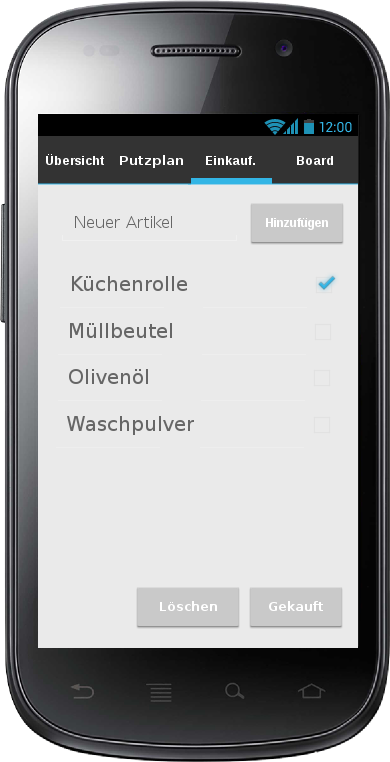
\includegraphics[width=0.7\textwidth]{anhang/mockups/einkaufsliste.png}
  \caption{Mockup Einkaufsliste - �bersicht}
  \label{anhang:mockEinkauf}
\end{figure}

\begin{figure}[H] 
  \centering
     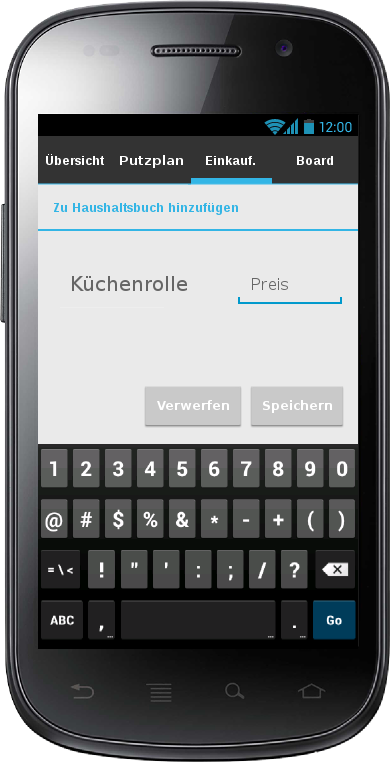
\includegraphics[width=0.7\textwidth]{anhang/mockups/einkaufslisteartikelgekauft.png}
  \caption{Mockup Einkaufsliste - Artikel gekauft}
  \label{anhang:mockEinkauf01}
\end{figure}

\begin{figure}[H] 
  \centering
     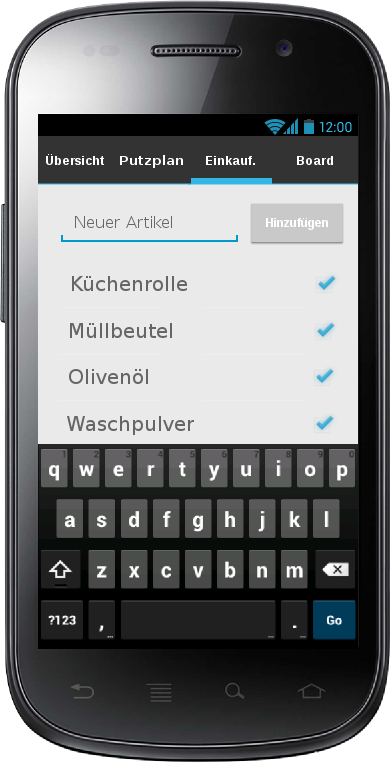
\includegraphics[width=0.7\textwidth]{anhang/mockups/einkaufslisteneuerartikel.png}
  \caption{Mockup Einkaufsliste - Neuen Artikel hinzuf�gen}
  \label{anhang:mockEinkauf02}
\end{figure}

\begin{figure}[H] 
  \centering
     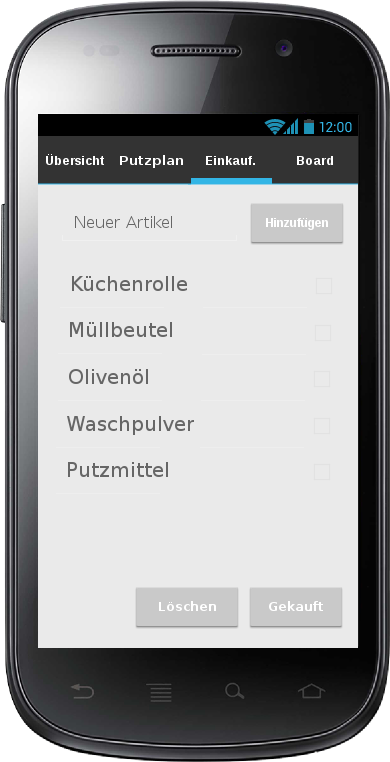
\includegraphics[width=0.7\textwidth]{anhang/mockups/einkaufslisteneuerartikelangefuegt.png}
  \caption{Mockup Einkaufsliste - Neuer Artikel hinzugef�gt}
  \label{anhang:mockEinkauf03}
\end{figure}

\begin{figure}[H] 
  \centering
     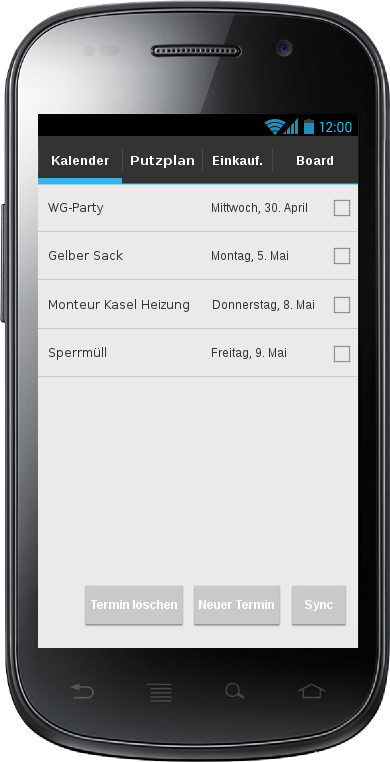
\includegraphics[width=0.7\textwidth]{anhang/mockups/kalender.png}
  \caption{Mockup Kalender - �bersicht}
  \label{anhang:mockKal}
\end{figure}

\begin{figure}[H] 
  \centering
     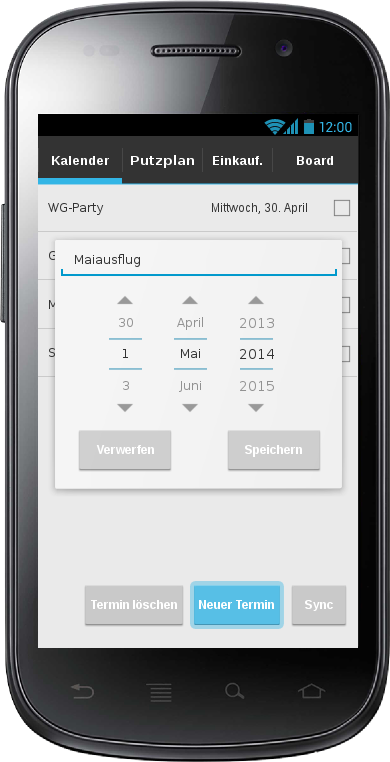
\includegraphics[width=0.7\textwidth]{anhang/mockups/kalenderneuertermin.png}
  \caption{Mockup Kalender - Neuer Termin}
  \label{anhang:mockKal01}
\end{figure}

\begin{figure}[H] 
  \centering
     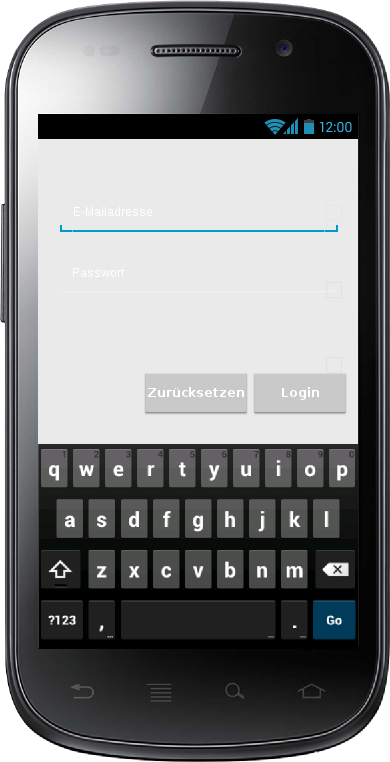
\includegraphics[width=0.7\textwidth]{anhang/mockups/login.png}
  \caption{Mockup Login}
  \label{anhang:mockLogin}
\end{figure}

\begin{figure}[H] 
  \centering
     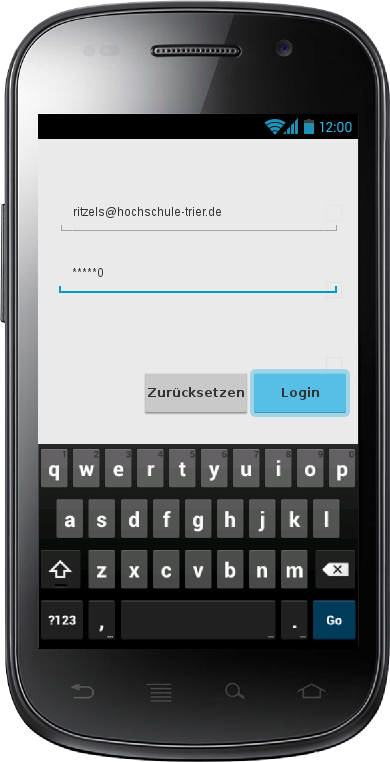
\includegraphics[width=0.7\textwidth]{anhang/mockups/loginnext.png}
  \caption{Mockup Login - Eingabe}
  \label{anhang:mockLogin}
\end{figure} 
    \begin{figure}[htbp] 
  \centering
     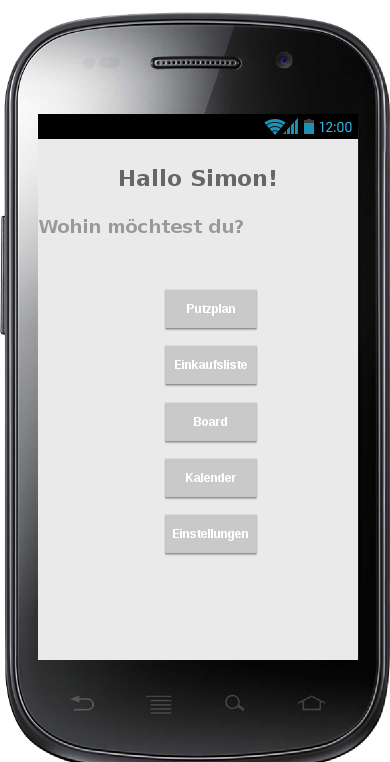
\includegraphics[width=0.7\textwidth]{anhang/mockups/overview.png}
  \caption{Erstes Bild}
  \label{fig:Bild1}
\end{figure}

\begin{figure}[htbp] 
  \centering
     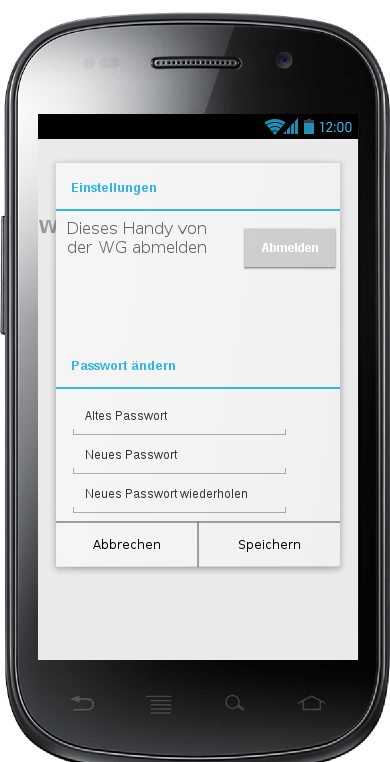
\includegraphics[width=0.7\textwidth]{anhang/mockups/overviewsettings.png}
  \caption{Erstes Bild}
  \label{fig:Bild1}
\end{figure}

\begin{figure}[htbp] 
  \centering
     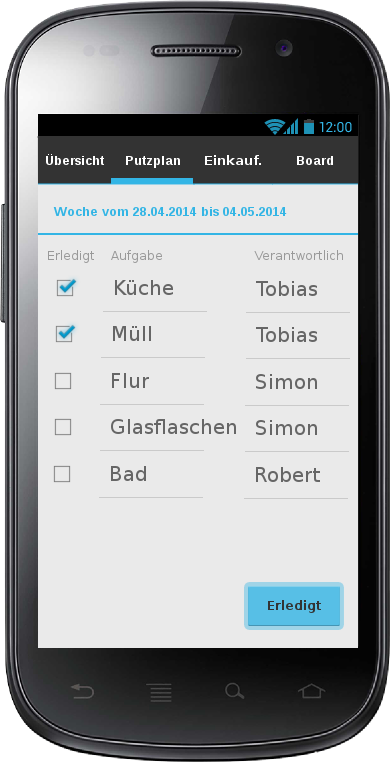
\includegraphics[width=0.7\textwidth]{anhang/mockups/putzplan.png}
  \caption{Erstes Bild}
  \label{fig:Bild1}
\end{figure}

\begin{figure}[htbp] 
  \centering
     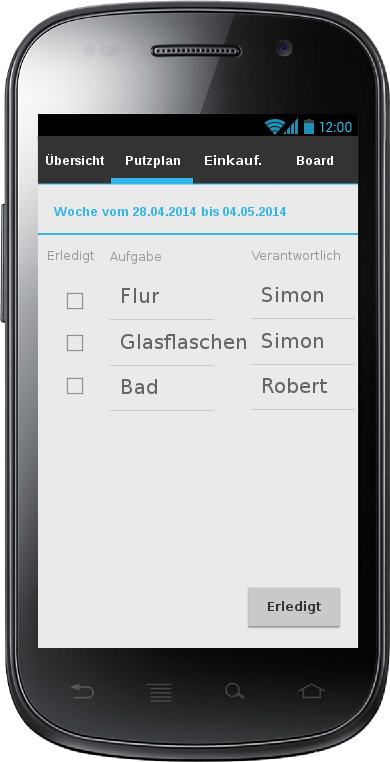
\includegraphics[width=0.7\textwidth]{anhang/mockups/putzplanerledigt.png}
  \caption{Erstes Bild}
  \label{fig:Bild1}
\end{figure}

\begin{figure}[htbp] 
  \centering
     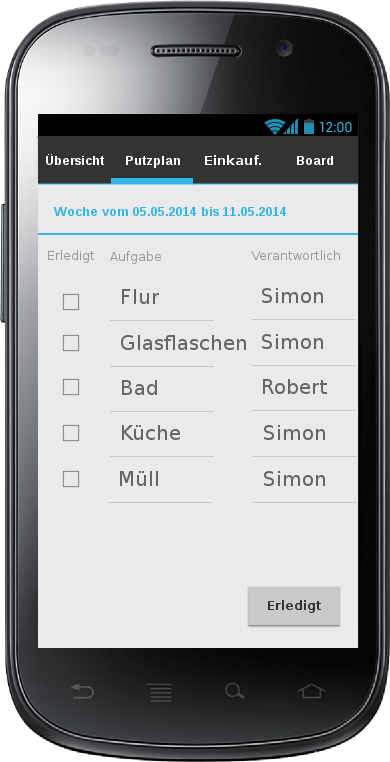
\includegraphics[width=0.7\textwidth]{anhang/mockups/putzplanneuewoche.png}
  \caption{Erstes Bild}
  \label{fig:Bild1}
\end{figure}

\begin{figure}[htbp] 
  \centering
     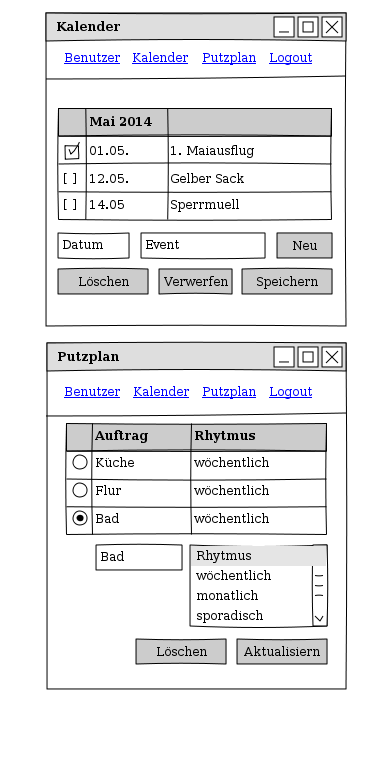
\includegraphics[width=0.7\textwidth]{anhang/mockups/webpage_1.png}
  \caption{Erstes Bild}
  \label{fig:Bild1}
\end{figure}

\begin{figure}[htbp] 
  \centering
     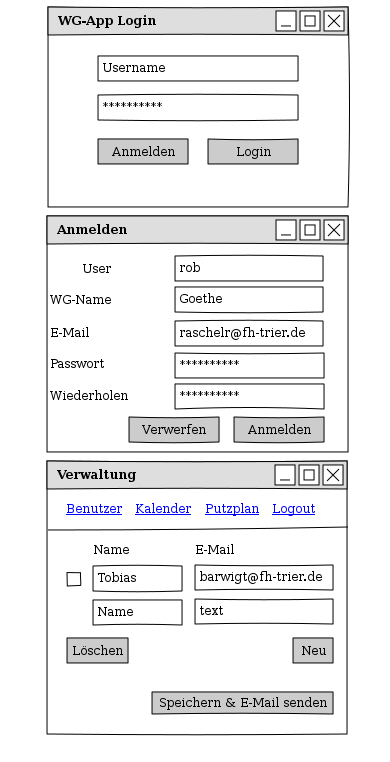
\includegraphics[width=0.7\textwidth]{anhang/mockups/webpage.png}
  \caption{Erstes Bild}
  \label{fig:Bild1}
\end{figure}

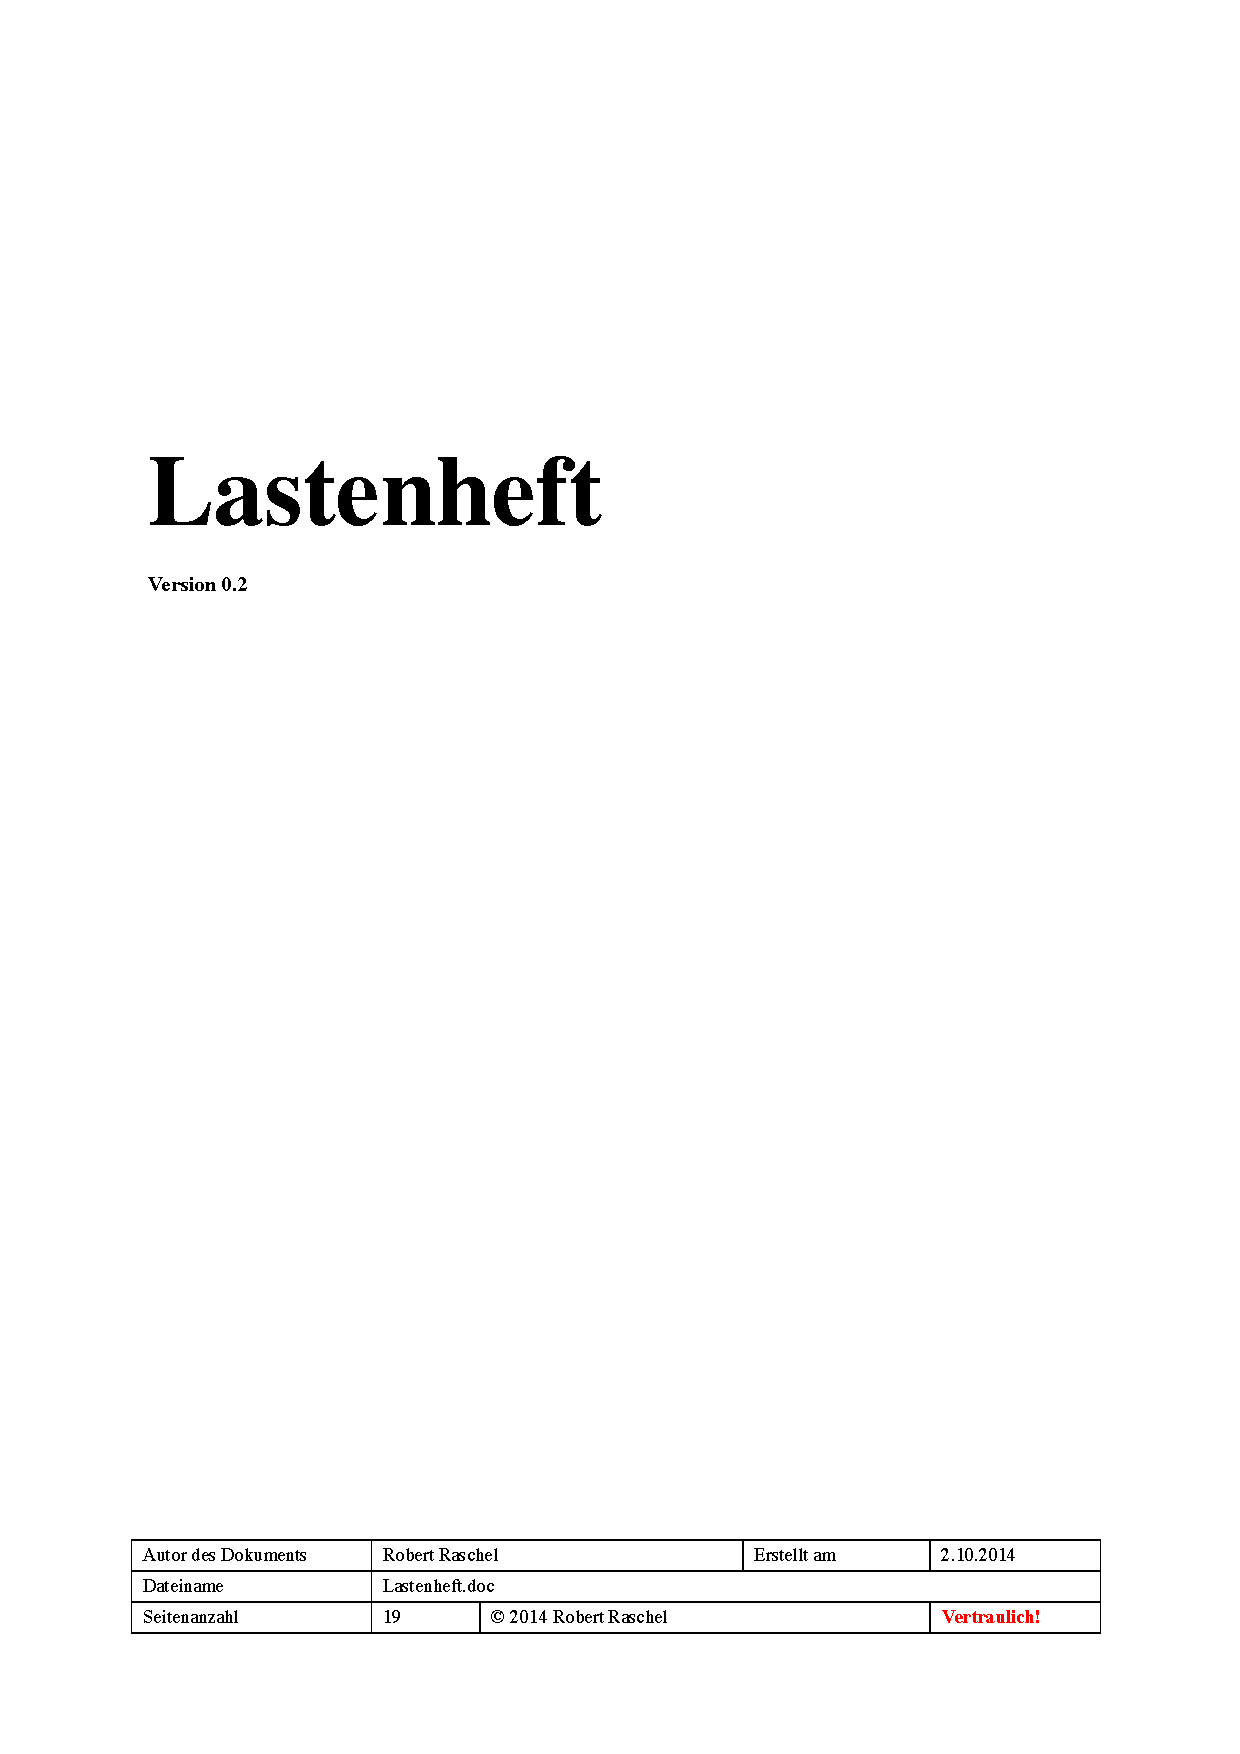
\includepdf[pages=-, addtotoc={1,chapter,0,Lastenheft,chap:int},  scale=0.85, pagecommand={}]{anhang/Lastenheft.pdf} 
%\includepdf[pages=2-, addtotoc={1,chapter,0,Lastenheft,chap:int},  scale=0.85, pagecommand={}]{anhang/Lastenheft.pdf} 


\end{appendix}

\end{document}
